\documentclass[12pt,a4paper]{article}
\usepackage[utf8]{inputenc}
\usepackage{amsmath}
\usepackage{amsfonts}
\usepackage{amssymb}
\usepackage{graphicx}
\graphicspath{ {images/} }
\usepackage{algorithm}
\usepackage[noend]{algpseudocode}
\usepackage{hyperref}
\usepackage[table,xcdraw]{xcolor}
\usepackage{subcaption}
\usepackage{colortbl}
\usepackage{hhline}
\hypersetup{
    colorlinks,
    citecolor=black,
    filecolor=black,
    linkcolor=blue,
    urlcolor=black
}


\newcommand\tab[1][1cm]{\hspace*{#1}}

\makeatletter
\def\BState{\State\hskip-\ALG@thistlm}
\makeatother

% Default fixed font does not support bold face
\DeclareFixedFont{\ttb}{T1}{txtt}{bx}{n}{12} % for bold
\DeclareFixedFont{\ttm}{T1}{txtt}{m}{n}{12}  % for normal

% Custom colors
\usepackage{color}
\definecolor{deepblue}{rgb}{0,0,0.5}
\definecolor{deepred}{rgb}{0.6,0,0}
\definecolor{deepgreen}{rgb}{0,0.5,0}

\usepackage{listings}

% Python style for highlighting
\newcommand\pythonstyle{\lstset{
language=Python,
basicstyle=\tiny ,
morekeywords={self},              % Add keywords here
keywordstyle=\tiny\color{deepblue},
emph={MyClass,__init__},          % Custom highlighting
emphstyle=\tiny\color{deepred},    % Custom highlighting style
stringstyle=\color{deepgreen},
frame=tb,                         % Any extra options here
showstringspaces=false
}}


% Python environment
\lstnewenvironment{python}[1][]
{
\pythonstyle
\lstset{#1}
}
{}

% Python for external files
\newcommand\pythonexternal[2][]{{
\pythonstyle
\lstinputlisting[#1]{#2}}}

% Python for inline
\newcommand\pythoninline[1]{{\pythonstyle\lstinline!#1!}}
\renewcommand{\contentsname}{Indice}

\begin{document}
\begin{titlepage}
	\centering
	{
\includegraphics[scale=0.5]{logo}\par}
	\vspace{1cm}
	{\bfseries\large ESCUELA TÉCNICA SUPERIOR DE INGENIERÍA INFORMÁTICA \par}
	\vspace{1cm}
	{\scshape\large DOBLE GRADO INGENIERIA DEL SOFTWARE + MATEMÁTICAS\par}
	\vspace{1cm}
	{\bfseries\large Curso Académico 2021/2022 \par}
	\vspace{1cm}
	{\bfseries\large  Trabajo Fin de Grado \par}
	\vspace{2cm}
	{\scshape\large DESARROLLO E INTERFAZ DEL ESTUDIO DE DIVERSIFICACIÓN DE INVERSIONES SOBRE IBEX-35 UTILIZANDO CLUSTERING\par}
	\vspace{2cm}
	\vfill
	{\normalsize\textbf Autor: \par}
	{\normalsize Javier Méndez García-Brioles \par}
	{\normalsize\textbf Directores: \par}
	{\normalsize Regino Criado \par}
\end{titlepage}





	\vspace{1cm}
	\tableofcontents

\pagebreak
	
	\vspace{1cm}
	\section{Resumen}
	\vspace{1cm}
Este proyecto tiene como finalidad explicar el desarrollo de los algoritmos e interfaz que permiten a \cite{Principal} proponer un plan de inversión alternativo para minimizar la volatilidad de la inversión, y por tanto, minimizar el riesgo.\\
El plan de inversión consiste en aplicar una modificación del algoritmo k-means para agrupar los stocks en k clusters y de esos clusters sacar un optimo, dando lugar a k stocks diferentes en los que invertir.\\
Con esté plan haremos un estudio sobre los stoks del IBEX-35 comparando nuestro algoritmo con planes de inversión convencionales para ver como se consigue la mínima volatilidad. Ademas haremos un estudio de previsión para ver si nuestro algoritmo mantiene la mínima volatilidad si añadimos datos posteriores a los que tiene como input el algoritmo.\\
Además facilitaremos una interfaz gráfica para mostrar e interactuar con los datos.\\
\pagebreak
	\vspace{1cm}
	\section{Objetivos}
	\vspace{1cm}
Desde siempre ha existido la necesidad de comparar datos y ver su relación entre ellos, y una muy buena forma de ejercer esta comparación es clasificando los estos datos en conjuntos de datos. Dentro de cada conjunto los datos tienen mayor relación entre ellos que con los datos de fuera del conjunto, pero la búsqueda de estos conjuntos no es fácil. En la actualidad a esta búsqueda se la denota como clustering, que es puede considerar como el proceso por el cual se crean conjuntos de elementos similares. Este proceso se puede aplicar sobre todo conjunto de datos sobre los que se pueda aplicar una comparación entre ellos pero en este caso nos centraremos en buscar clusters de ondas temporales mediante varios métodos que comentaremos a continuación.\\
En un principio nos íbamos a basar en el grafo de visibilidad sacado de cada stock para, mediante sus propiedades, agrupar estos stocks. Pero al decidirnos por agrupar los stocks mediante k-means, la transformación a grafo de visibilidad ha pasado a un segundo plano, sirviendo como medio para transformar nuestras series iniciales a otras series que recojan las propiedades de los grafos de visibilidad.\\
Partimos de un conjunto de elementos, los cuales están compuestos por una sucesión de valores a lo largo de un intervalo de tiempo, estos elementos se pueden clasificar tal cual, o se puede hacer una transformación antes de su clasificación y utilizar esa transformación como input. En nuestro caso exploraremos 3 caminos:\\
1 Realizamos la clasificación sobre los elementos sin transformar.\\
2 Transformamos los elementos en una versión simplificada de ellos mismos para intentar mejorar el tiempo de ejecución.\\
3 Transformamos los elementos en su correspondiente grafo de Visibilidad y luego aplicamos el algoritmo sobre esos grafos.\\
Este proyecto se basara en la clasificación de series temporales mediante una variación sobre un método muy conocido llamado K-Means, lo que nos permite clasificar elementos siempre que se pude definir una función distancia entre ellos.\\
Una vez que tenemos nuestros elementos separados en distintos conjuntos, después de hacer las transformaciones y aplicar el algoritmo K-means tenemos k conjuntos cuyos elementos son similares entre ellos, esto resulta muy útil ya que nuestros elementos de entrada son stocks, por lo tanto saber que stocks se parecen entre ellos nos permite evitar elegir stocks que se comportan de forma parecida lo que nos permite minimizar la volatilidad de la inversión.
Por último, una vez llegado al resultado que es la volatilidad de la inversión podremos comparar todos los caminos que hemos utilizado entre ellos y con resultados de control (como son invertir de forma homogénea en todos los stocks, invertir todo en el stock menos volátil o invertir en n stocks aleatorios) para ver así que variación del método es el mejor o si los resultados de control son superiores.\\
Durante todo el proyecto trabajaremos sobre los datos producidos por las empresas dentro del IBEX-35 y proporcionados por una API de yahoo finances.\\
Desde un punto de vista más teórico nos centraremos en evolucionar el algoritmo K-means para que se adecue a nuestras necesidades, lo que consiste en hacer modificaciones para que el K-means acepte distancias un poco menos convencionales que la genérica, ejecutar el K-means varias veces para mejorar la precisión de los conjuntos y por ultimo modificar K-means para que también funcione sobre un grafo.\\


	\vspace{1cm}











	\vspace{1cm}
	\section{Fundamentos Teóricos}
	\vspace{1cm}
		\subsection{Ondas Temporales}
			{\textbf{Ondas Simples}}\\
			Llamaremos ondas simples a las cuales compuestas exclusivamente por una función seno, con sus posibles modificaciones de amplitud, frecuencia, y desplazamiento.\\
			{\textbf{Ondas Compuestas}}\\
			Llamaremos ondas compuestas a la superposición de ondas simples a lo largo del tiempo\\
			{\textbf{Transformada de Fourier}}\\
			La transformada de Fourier es una función matemática que permite relacionar un dominio temporal con un dominio de frecuencias en ambos sentidos\\
			{\textbf{Transformada Wavelet}}\\
			La transformada Wavelet es una función muy utilizada en compresión de imágenes que permite dividir la cantidad de valores manteniendo la mayor cantidad posible de detalle.\\
		\subsection{Teoría de Grafos}
			{\textbf{Grafo}}\\
			Un grafo  ($G = (V,E)$) es una estructura de datos compuesta por vértices ($V$), donde se almacenan los datos, y aristas o arcos ($E=V\times V$), que representan las conexiones entre dos vértices.\\
			{\textbf{Grafo no Dirigido}}\\
			Grafo  ($G = (V,E)$) tal que:
			\[ V \neq \emptyset \]
			\[ E\subseteq \{ (a,b) / (a,b)\in E \rightarrow (b,a)\in E  \}  \]
			{\textbf{Vértice}}\\
			Componente mínimo indivisible por el que están compuestos los grafos\\
			{\textbf{Arista}}\\
			Componente de un grafo que se caracteriza por conectar dos vértices (E)\\
			{\textbf{Grado}}\\
			El grado de un vértice ($v\in V$) es:
			\[degre(v)=|E_v|\]
			\[ E_v\subseteq \{ (a,b)\in E / a=v \lor b=v \}  \]
			{\textbf{Orden}}\\
			El orden de un grafo ($G = (V,E)$) es:
			\[orden(G)= degre(w)\]
			con\\
			\[ w\in V / \forall v\in V      degre(w) \geq  degre(v)  \]
			{\textbf{Grafo de Visibilidad}}\\
			Un grafo de visibilidad es el grafo asociado a una onda temporal siguiendo el siguiente proceso:\\
			-A cada valor de la onda se le asigna un nodo del grafo.\\
			-Las conexiones se deciden según que nodos se ven entre ellos sin que otro nodo les bloque la visión. Esta restricción equivale a cumplir la ecuación ($y_m + \frac{y_n-y_m}{n-m}(k-m) \geq y_k$) para todo nodo k entre m y n ($ m < k < n$)\cite{GrafoVisibilidad} \\

		\subsection{Centralidad}
			La centralidad en un grafo consiste en la asignación de un número a cada nodo del grafo, este valor es sumamente importante ya que permite comparar nodos entre sí.\\
			La importancia de la centralidad reside en que encontrando nodos con valores muy altos de centralidad es equivalente a encontrar los nodos más importantes del grafo, los cambios a estos nodos causarán el mayor impacto dentro del grafo. Este valor es externo al propio nodo y puede variar con cualquier modificación del grafo, aunque esa modificación no afecte al grafo en sí.\\
			La centralidad es de suma importancia pues nos permite estudiar las conexiones entre objetos, ya sea entre personas a través de medios como las redes sociales, o las conexiones por carretera entre ciudades. Y este estudio por ejemplo nos permite saber la influencia de cierta persona x, o el trafico probable en una ciudad.\\
			Hay varias medidas que se pueden usar para determinar la centralidad, pero nosotros nos vamos a centrar en la centralidad de grado y la interpolación(Betweenness)\\
			{\textbf{Centralidad de grado}}\\
				La centralidad de grafo es posiblemente la medida de centralidad más fácil de entender. Consiste en contar el número de conexiones que tiene cada nodo, lo cual nos basta para ver si un nodo esta incomunicado o cual es la distancia entre cualquier pareja de nodos del grafo. Estos son datos muy útiles para el estudio de grafos, pero para ciertas aplicaciones se nos quedan cortos.\\ 
			{\textbf{Intermediación}}\\
				La intermediación es un poco más compleja y consiste en calcular el numero de veces que un nodo se utiliza como puente en la ruta más corta entre una pareja de nodos. Pongamos el ejemplo de una red de ordenadores, el nodo con una intermediación más alta seria por el cual pasa más información, sabiendo esto podemos ver que si ese nodo se incapacita sería el que más problemas ocasionaría a la red. Por lo tanto, con esta información podríamos saber los nodos que necesitan más protección en todo momento, esto es algo que con un simple estudio del grado de cada nodo no se vería.\\

		\subsection{Distancias}

		Una distancia es cualquier función que cumple lo siguiente:\\
			\begin{enumerate}
			\item $d(x,y) = 0 \iff x = y $
			\item $d(x,y) =d(y,x)$ (simetría)
			\item $d(x,z) \leq d(x,y) + d(y,z)$ (desigualdad triangular)
			\end{enumerate}
			Lo que nos dice de forma análoga por la desigualdad triangular:\\
			$d(x,y)\geq 0$ (no negatividad)\\

		\subsection{Volatilidad}
		La volatilidad es un termino que mide la variación de los valores a lo largo del tiempo, a mayor variación mayor volatilidad. Nuestra definición especifica de volatilidad va a ser bastante estándar.\\
		Definimos volatilidad como:\\
		\[Volatilidad = \sum_{i=1}^{n} \sqrt{\left | valor_i - media \right |} \]

		\subsection{Complejidad Computacional }
		Toda la teoría de Complejidad Computacional consiste en hacernos la pregunta, ¿que tareas son fáciles y que tareas son difíciles para un ordenador?. Al hacernos esta pregunta nos damos cuenta de no hay forma fácil de responder con lógica convencional ya que una tarea fácil para un ser humano no equivale a una tarea fácil para un ordenador. Pongamos como ejemplo reconocimiento de imágenes, si tenemos una imagen de un perro y se la enseñamos a una persona sabrá al momento que es un perro aunque no haya visto nunca esa foto exacta. \\
Pero para un ordenador eso resultaría imposible sin un gran trabajo por detrás y aunque en la actualidad ya existen algoritmos que permitan responder esa pregunta no están ni de lejos a la altura de una persona. \\
A su vez si tenemos cualquier tarea de computación pura un ordenador tardará mucho menos que  una persona. Así que resumiendo hay tareas fáciles para personas que nos casi imposibles para ordenadores y tareas fáciles para ordenadores que son casi imposibles para personas. \\
Por lo tanto para llegar a alguna conclusión vamos a necesitar una estrategia precisa que nos facilite algún indicador de que tareas son fáciles para un ordenador y eso es lo que hace el estudio de la Complejidad Computacional.\\
		 El estudio de la Complejidad se basa principalmente en estudiar dos parámetros, la cantidad de memoria utilizada por un algoritmo, y el numero de instrucciones que se ejecutan, esto equivale a medir el espacio y tiempo que gasta un algoritmo. Nosotros solo nos vamos a centrar en el estudio del tiempo.\\
		 
		Para un algoritmo concreto podemos definir la siguiente función T(n) a la cual le pasamos un input de tamaño n y nos devuelve el número de operaciones que realiza el algoritmo en el peor de los casos.\\
		\[T: N \rightarrow R^+ \]
		Como un ordenador realiza estas operaciones muy rápido los errores de magnitud pequeña pueden ser ignorados haciendo que solo nos importe el comportamiento asintótico de la ecuación conforme n crezca. Para expresar esto utilizaremos las siguientes definiciones.\\
		Sean $T, S : N \rightarrow R^+$ se dice que T(n) \textbf{domina} a S(n) si existen $k > 0$ y $n_o$ tal que para todo $n>n_0$:\\
		\[S(n) \leq kT(n) \]
		Con O(T(n)) siendo el conjunto de funciones dominadas por T(n) podemos decir que dos funciones T(n) y S(n) son \textbf{del mismo orden} si $ S(n) \in O(T(n)) y T(n) \in O(S(n))$.\
		Se llama \textbf{complejidad de un algoritmo} al mayor orden O(n) al que pertenece T(n).\\ 
		Dependiendo de cual sea el mayor O(n) al que pertenece T(n) podemos hablar de distintas complejidades. 
			\begin{enumerate}
			\item Con $T(n) \in O(log(n))$ se dice que el algoritmo tiene \textbf{complejidad logarítmica}
			\item Con $T(n) \in O(n)$ se dice que el algoritmo tiene \textbf{complejidad lineal}
			\item Con $T(n) \in O(n^2)$ se dice que el algoritmo tiene \textbf{complejidad cuadrática}
			\item Con $T(n) \in O(n^x)$ se dice que el algoritmo tiene \textbf{complejidad polinomial}
			\item Con $T(n) \in O(e^n)$ se dice que el algoritmo tiene \textbf{complejidad exponencial}
			\end{enumerate}
		

		\subsection{Algoritmos}
		{\textbf{Algoritmo de Dijkstra}}\\
		También conocido como algoritmo de mínimos caminos nos permite determinar el camino más corto entre un nodo origen y el resto de los nodos del grafo, si se hace este algoritmo sobre todos los nodos nos queda como resultado la mínima distancia entre todos los pares de nodos. Aquí se muestra su pseudocódigo:\\
			    \begin{algorithm}[H]
			    \caption{Algoritmo de Dijkstra}\label{euclid}
			    \hspace*{\algorithmicindent} \textbf{Input: {\normalfont   Grafo} ${G = (V,E)} $}\\
			    \textbf{\tab \tab {\normalfont \quad Nodo inicial}  ${node\_init}$}\\
			    \hspace*{\algorithmicindent} \textbf{Output:{\normalfont \quad Distancias} $\mathcal{D}=\{d_1..d_n\}$} 
			    \begin{algorithmic}[1]
			    \Procedure{Dijkstra}{${G},node\_init$}
			    \BState $\mathcal{D}=\{ d_1..d_n \} \gets \{INF..INF\}$
			    \BState ${pred} \gets \{\emptyset..\emptyset\}$
			    \BState ${seen} \gets \{False..False\}$
			    \BState ${D[node\_init]} \gets 0$
			    \BState \# \textit{Utilizamos una cola para asegurar el recorrido total del grafo}
			    \BState Q.add(node\_init,D[node\_init])
			    \BState \textbf{while}  ${Q \neq \emptyset }  \textbf{ do}$:
			    \State \# \textit{Extraer elemento de mínima distancia}
			    \State $node \gets Q.min()$
			    \State $seen[node] \gets True$

		            \For{$v \in adjacent(node)$} \do
			    \State \State 	\# \textit{Añadimos distancia si es menor que la actual}
				    \If {(\textbf{not} seen[v] \textbf{and} $\mathcal D[v] > \mathcal D[node] + E[node,v]$ )}
					\State $\mathcal D[v] \gets \mathcal D[node] + E[node,v]$
					\State $pred[v] \gets node$
			    		\State Q.add(v,D[v])
				    \EndIf
		            \EndFor
			    \BState \textbf{return} D;
			
			    \EndProcedure
			    \end{algorithmic}
			    \end{algorithm}
		Este algoritmo tiene una complejidad computacional $\mathbf{O(n^2)}$ ya que para cada nodo se puede llegar a recorrer todos los nodos. Pero si queremos saber las distancias entre todos los nodos la complejidad computacional aumenta a  $\mathbf{O(n^3)}$ pues hay que ejecutar el algoritmo de Dijkstra para cada nodo.\\
		{\textbf{K-means}}\\
		El K-means o K-medias es un método de clasificación no supervisada que permite la clasificación de n elementos en k grupos distintos, en cada uno de estos k grupos los elementos dentro se consideran más parecidos entre ellos que con los elementos de fuera. K-means se centra en resolver un problema de optimización en el cual se busca minimizar la suma total de la distancia de los elementos a su centroide más cercano:
		\[\min_{C} \sum_{i=1}^{k}\sum_{x_{j}\in C_{i}} d(\sigma_i , x_{j})\]
		Donde $d(x,y)$ es la función distancia utilizada,  $\{x_1..x_n\}$ son los elementos, $C=\{C_1..C_k\}$ son los k clusters y $\{\alpha_1..\alpha_k\}$  son los centroides correspondientes a cada cluster.\\
			La principal ventaja del k-means es que es muy rápido, pero tiene también una gran desventaja que hay que tener en cuenta, los resultados obtenidos dependen enormemente de como se inicializan los centroides. Por esta razón no podemos asegurar un optimo global sino que nos tendremos que conformar con un optimo local.\\
			K-means consta de 3 partes indispensables:\\
			\begin{enumerate}
			\item \textbf{Inicialización de centroides}: Se determinan las posiciones iniciales de los centroides, esto se puede hacer de muchas formas, todas ellas validas y todas ellas pueden dar soluciones ligeramente distintas. Podemos elegir por ejemplo los k primeros elementos como centroides o elegirlos de forma aleatoria.\\
			\item \textbf{Relacionar cada elemento con un centroide}: Para cada elemento se calcula la distancia a todos  los centroides y se relaciona con el centroide más cercano. Cada elemento se añade al cluster del centroide correspondiente.\\
			\item \textbf{Actualizar centroides}: Se actualizan los centroides haciendo la media de todos los elementos de su cluster y ese valor es el nuevo centroide.\\
			\end{enumerate}
			Los pasos 2 y 3 se repiten hasta que llegamos a nuestra condición de parada, que suele ser que la diferencia entre los centroides anteriores y los nuevos centroides sea menor a un valor umbral.\\
			
			El proceso se puede ver con más detalle en el siguiente pseudocódigo:\\
\pagebreak
			    \begin{algorithm}
			    \caption{K-means clustering}\label{euclid}
			    \hspace*{\algorithmicindent} \textbf{Input: {\normalfont   Data} $\mathcal{X} = \{x_1..x_n\}$}\\
			    \textbf{\tab \tab {\normalfont \quad Numero de clusters}  ${k}$}\\
			    \textbf{\tab \tab {\normalfont \quad Valor umbral}  ${ \varepsilon }$}\\
			    \hspace*{\algorithmicindent} \textbf{Output:{\normalfont \quad Clusters} $\mathcal{C}=\{C_1..C_k\}$} 
			    \begin{algorithmic}[1]
			    \Procedure{K-means}{$\mathcal{X},k,\varepsilon$}
			    \BState $\mathcal{C}=\{C_1..C_k\} \gets \{\emptyset..\emptyset\}$
			    \BState $ \{\sigma_1..\sigma_k\}  \gets$ \textbf {InicializarCentroides}($\mathcal{X},k$)
			    \BState \textbf{loop}:
			    \State \# \textit{Distribución de elementos en clusters}
			    \State $C_i \gets \{x_j / d(\sigma_i,x_j)  \leq d(\sigma_h,x_j) \forall h  \in \{1..k\}  \}  \forall i  \in \{1..k\}$
			    \State \# \textit{Actualización de clusters}
			    \State $new\sigma_i \gets \frac{\sum_{x_j\in C_i}x_j}{|C_i|} \forall i  \in \{1..k\}$
			    \State \# \textit{Comprobar la condición de parada}
			    \If {($ \sum_{i=1}^{k} d(\sigma_i,new\sigma_i) \leq  \varepsilon$)}
			    \State \Return $\mathcal{C}$
			    \EndIf
			    \State $ \{\sigma_1..\sigma_k\}  \gets \{new\sigma_1..new\sigma_k\}$
			    \State \textbf{goto} \emph{loop}.
			    \BState \textbf{close};
			    \EndProcedure
			    \end{algorithmic}
			    \end{algorithm}
			Para este algoritmo es difícil estudiar su complejidad computacional ya que el camino para llegar a la condición de parada es difícil de definir, por eso mismo se le considera un problema computacionalmente difícil (NP-hard), se han demostrado cotas de su complejidad como $\mathbf{O(n^{34}k^{34}d^8 log^4(n)/\sigma^6) }$ o $\mathbf{O(dn^4M^2)}$ para casos más simples, pero nosotros nos referiremos a su complejidad como $\mathbf{O_{K-means}}$ para poder compárala con la complejidad de las modificaciones al algoritmo\\


\subsection{Terminos de desarrollo Software}
{\textbf{Herencia}}\\
	La Herencia es un concepto software utilizado para facilitar la extension y mantenimiento del software abstrayendo los puntos comunes de varias clases en una clase común. Se dice que estas clases derivan de la clase común.\\
{\textbf{Requisitos}}\\
	Los requisitos contienen las expectativas de la parte de negocio hacia el proyecto software. Son las metas hacia las que llevar el desarrollo software para general valor al cliente.\\
{\textbf{Valor}}\\
	Se considera como Valor a la ganancia, material o conceptual, que se genera al implementar los requisitos en un proyecto software, este concepto se suele tener en cuenta en la priorización de requisitos.\\
{\textbf{Tareas}}\\
	Las tareas son cada uno de los elementos donde se recogen los requisitos para crear valor, es decir, añadir funcionalidad al proyecto. Cada requisito se suele dividir en varias tareas dependiendo del tamaño del mismo.\\
{\textbf{WIP}}\\
	WIP representa las siglas de "Work in Progress" y se utiliza para limitar las tareas que están en desarrollo en un instante de tiempo, si tenemos un WIP de 4 no se recomienda que se tengan más de 4 tareas abiertas en cada momento.\\


\pagebreak
	\vspace{1cm}
	
	
	\vspace{1cm}
	\section{Herramientas}
	\vspace{1cm}
Para este proyecto crearemos una aplicación python mediante la cual interactuaremos con la funcionalidad implementada, para esta implementación utilizaremos las siguientes herramientas:\\
\subsection{Anaconda}
Anaconda es una plataforma que gestiona entornos python para facilitar la instalación y uso de librerías python. Anaconda se centra en facilitar la programación científica, lo que incluye ciencia de datos, aprendizaje maquina y procesado de datos. Esto lo consigue implementando otra forma de instalar librerías a través del comando conda que equivale a el pip normal de python pero se centra en prevenir conflictos en la instalación de librerías, lo que produce un entorno más resistente a fallos de compatibilidad de librerías que con python convencional.\\
\subsection{Spyder}
Spyder es el IDE (Entorno de desarrollo integrado) que utilizaremos para la mayor parte de la programación. Viene por defecto con una gran cantidad de librerías integradas que resultan muy útiles para el desarrollo de código científico, como puede ser numpy o pandas. Ademas como es un entorno de código abierto, es decir, que permite que cualquiera pueda cambiar y distribuir el código, lo que hace que tenga una gran variedad de extensiones muy útiles para el desarrollo software.\\
\subsection{Extensiones Integradas en Spyder}
Aquí mencionaremos las principales extensiones que se han utilizado en el desarrollo de este proyecto:\\
-Spyder-Unittest: Es una extensión sobre Spyder que permite la automatización de test unitarios sobre nuestro código, ademas esta funcionalidad viene con una interfaz propia que permite la ejecución de todos los tests implementados a la vez y así poder ver al momento cuales fallan y cuales pasan.\\
-Spyder-GitHub: Es una extensión que permite acceder a GitHub desde dentro del entorno de desarrollo Spyder, lo que proporciona una pequeña interfaz gráfica para hacer commits y ver el historial del repositorio, ademas de permitir el uso de los comandos git dentro del terminal de Spyder.\\
-Spyder-Code Análisis: Esta extensión no da información sobre la calidad del código, muestra tanto las diferencias con las convenciones de como programar en python como las warnings y las vulnerabilidades del código.\\
-Spyder-Profiler: Esta extensión simplemente permite ver como está distribuido el tiempo de ejecución de la aplicación. El tiempo de ejecución se separa por método, lo que permite ver que métodos están consumiendo más recursos y esto ayuda en el proceso de optimización del código.\\
\subsection{Qt Designer}
Qt Designer es una herramienta que facilita el diseño de aplicaciones python aportando entorno donde poder crear, ver y gestionar la interfaz de una aplicación python. Este interfaz que se crea aquí se pude convertir en código python, el cual a su vez puede ser modificado en cualquier entorno de desarrollo python para añadir funcionalidad real a la aplicación. Qt Designer permite el uso de la librería gráfica QT en python lo que nos da opciones útiles que no nos dan otras librerías de interfaces de python como puede ser tkinter.\\
\subsection{Trello}
Trello es una aplicación con acceso web que permite la administración de proyectos. Se basa en un modelo kanban para poder llevar un seguimiento de las tareas a realizar en el desarrollo de nuestra aplicación.\\
\subsection{Github}
Github es un sistema de control de versiones que permite tener el código subido a un repositorio mientras que los cambios se hacen en local. Esto si se hace bien ayuda mucho en el desarrollo del código porque nos permite compartimentar cada parte de la funcionalidad en un commit individual que explique lo que se ha implementado en el mismo. Esto permite tener un buen historial de desarrollo para mejorar la mantenibilidad del código y permite tener versiones de código anteriores en caso de que durante el desarrollo rompamos la versión que tenemos del código en local y no sepamos arreglarlo, en este caso siempre podemos volver a la versión anterior del código para solucionar el problema.\\
\subsection{GitMind}
Este programa nos permite la creación de diagramas UML (lenguaje unificado de modelado) para poder mostrar una gran cantidad de relaciones distintas, por ejemplo la relación de las clases de nuestro programa, los casos de uso desde el punto de vista de un usuario o el diagrama de flujo que sigue el programa. Este programa tiene el problema de que solo exporta los diagramas de forma fidedigna en formato .svg, asi que para la memoria los transformo en .png, pero se pueden encontrar los diagramas en formato .svg en los apéndices.\\
\subsection{LaTex}
Sistema de composición de textos que permite  la creación de documentos en formato estructurado y con eso se facilita el uso de elementos matemáticos y pseudocódigo en la memoria.\\
\pagebreak

	\section{Metodología}
	Durante todo este proyecto vamos a explicar el desarrollo del código que habilita la funcionalidad de \cite{Princial} y para ello antes de nada vamos a explicar la metodología que se seguirá en todo el desarrollo.\\
	\subsection{Agilidad}
	Utilizaremos los que se conoce como metodología ágil para realizar este proyecto, la metodología ágil se lleva usando desde el principio del desarrollo software, pero no fue hasta el 2001 que se formalizó a través del Manifiesto Ágil, el cual da una serie de pautas o consejos para el desarrollo de software ágil. La metodología ágil se basa en implementar un proceso iterativo e incremental en el desarrollo de la funcionalidad del proyecto, a diferencia del modelo en cascada que es más rígido y difícil de iterar en intervalos cortos de tiempo.\\
	
\begin{figure}[H]
\centering
  \centering
  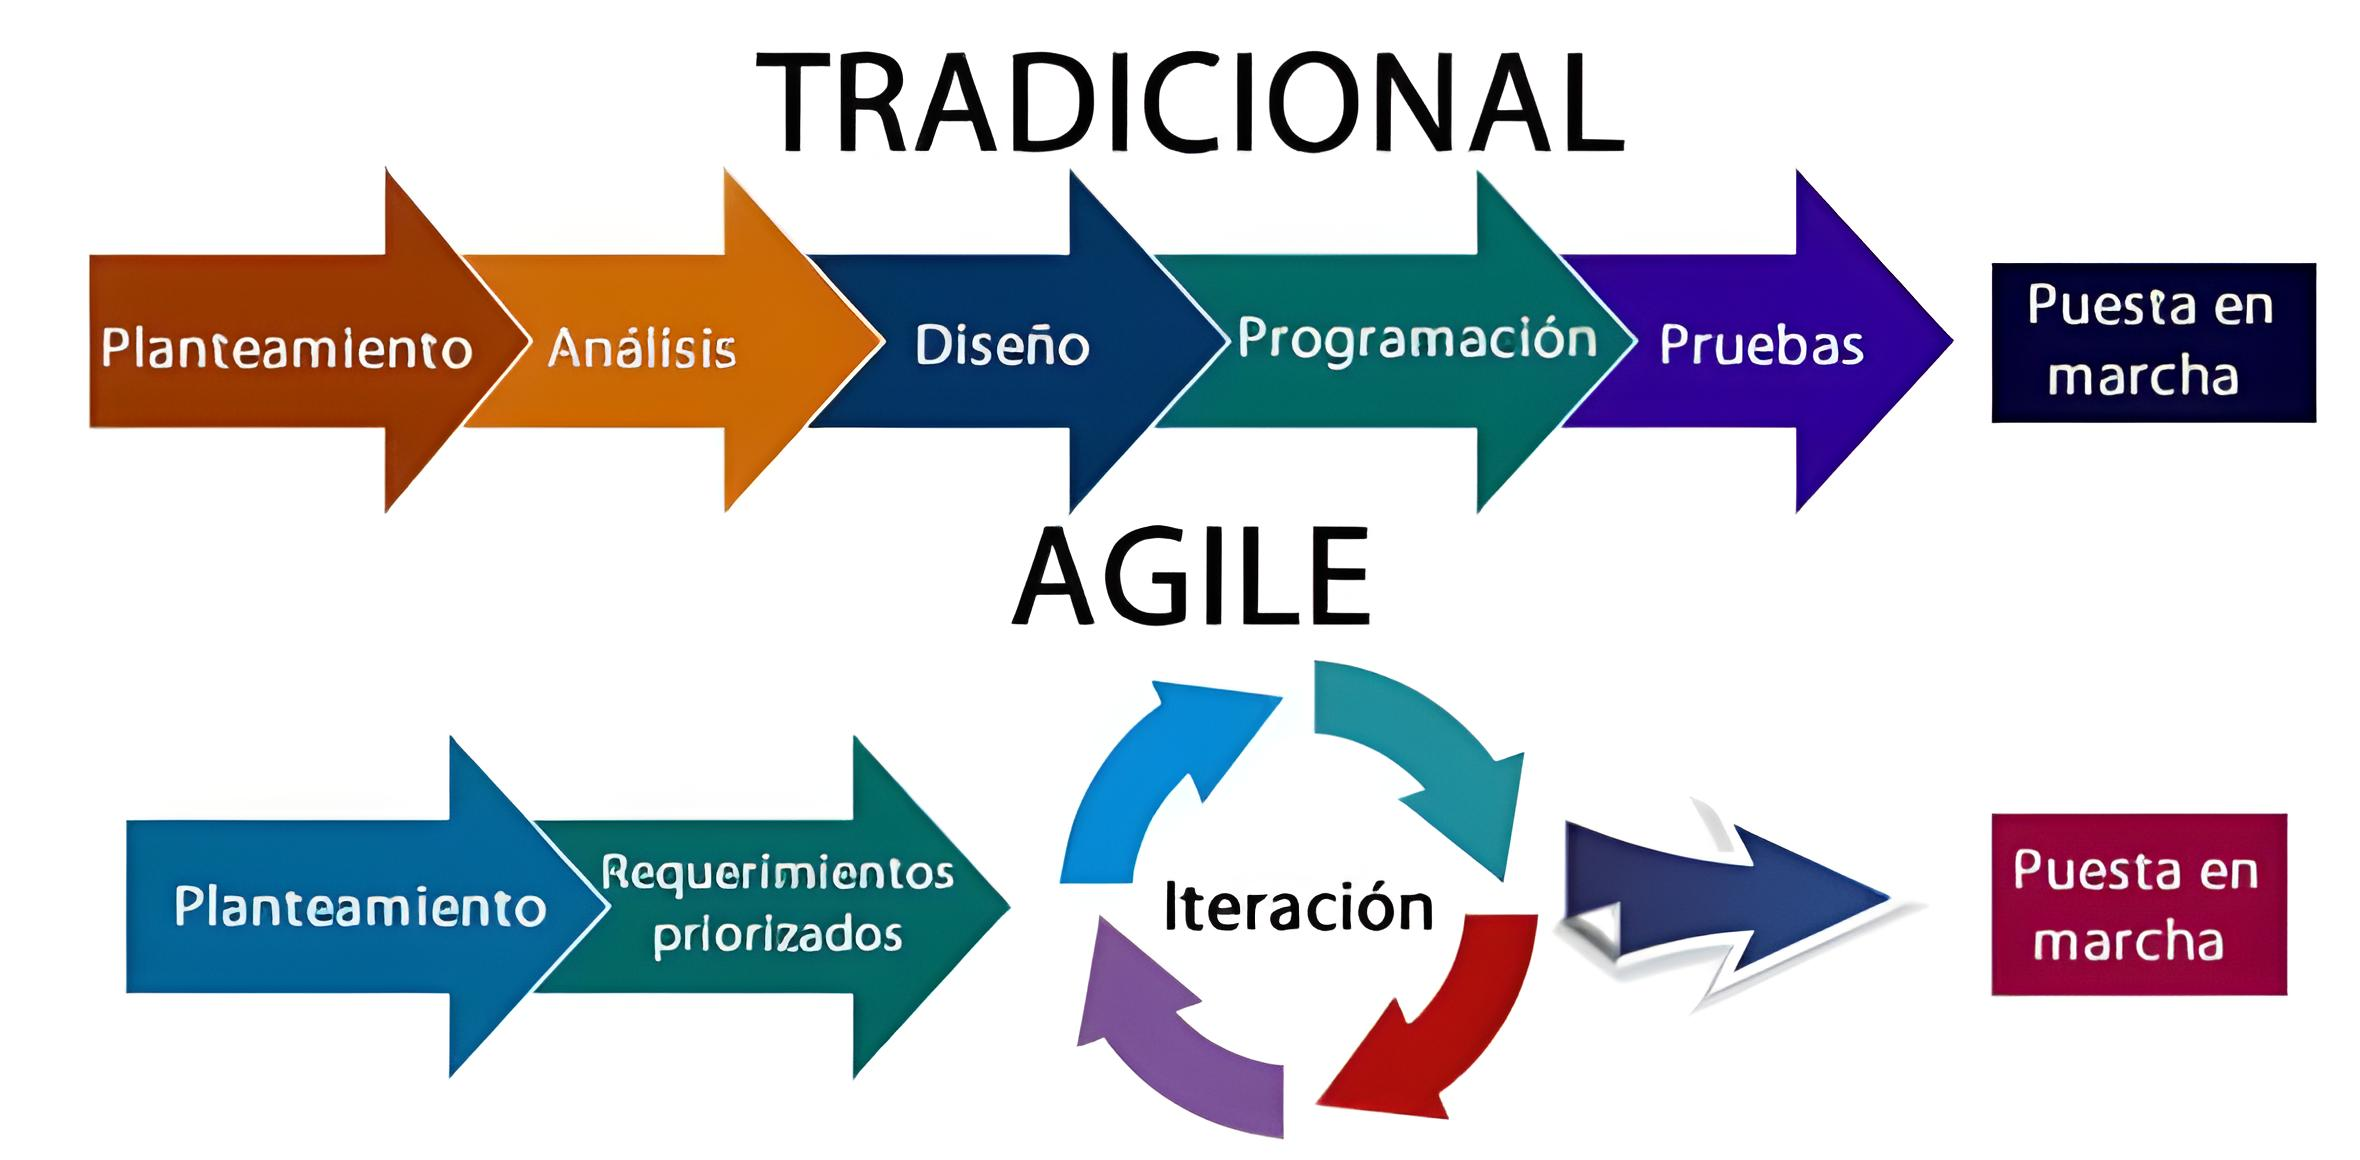
\includegraphics[width=0.5\linewidth]{metodologias}
\caption{Comparacion metodologia tradicional / metodologia agil}
\label{fig:subrgrafo}
\end{figure}

	El enfoque ágil es recomendable en el desarrollo de proyectos software, ya que a diferencia de proyectos físicos en los proyectos software los cambios de diseño tienen un coste muy limitado. Esto facilita las modificaciones a lo largo del desarrollo que es lo que propone la metodología ágil.\\
	En nuestro caso el uso de esta metodología no va a tener tanto impacto como podría ya que de desarrollo del proyecto lo va a realizar una sola persona. Esto quiere decir que la implementación de técnicas de organización del proyecto tendrán impacto limitado, aun así la implementación de estas practicas merecerá la pena a largo plazo.\\
	
	\subsection{Tablero Kanban}
	Posiblemente la practica más significativa en el desarrollo de un proyecto ágil consiste en la creación de un Tablero Kanban. Este tablero es una herramienta que permite visualizar el fujo de trabajo del proyecto.\\
\begin{figure}[H]
\centering
  \centering
  
\includegraphics[width=0.5\linewidth]{kanban generico}
\caption{Tabla Kanban basica con un WIP de 2}
\label{fig:subrgrafo}
\end{figure}
	La composición como podemos ver en la imagen anterior consiste en dividir el tablero en columnas, cada una de estas columnas contienen las tareas repartidas dependiendo de su estado actual.\\
	\begin{enumerate}
	\item La columna TO DO contiene las tareas que ya han sido formuladas como requisitos que tiene que cumplir el código pero todavía no se ha empezado a trabajar en ellas.
	\item La columna IN PROGRESS contiene las tareas cuya funcionalidad se esta incluyendo en el proyecto en estos momentos, vemos que esta columna tiene un WIP de 2 lo que indica que el máximo número de tareas que puede contener en cada momento es 2, esto se hace para reducir el número de tareas abiertas, lo que mejora la productividad.
	\item La columna DONE contiene las tareas que ya han sido implementadas en el proyecto.
	\end{enumerate}
	 El Tablero Kanban, si le usamos en un entorno ágil, permite ser customizado como mejor convenga al equipo de desarrollo. Por ejemplo, si estamos hablando de un proyecto grande puede que convenga añadir otra columna entre IN PROGRESS y DONE que podemos llamar por ejemplo VALIDATION que pueda contener las tareas que ya están terminadas pero requieren confirmación de otro miembro del equipo para que se cierren.
	\begin{figure}[H]
\centering
  \centering
  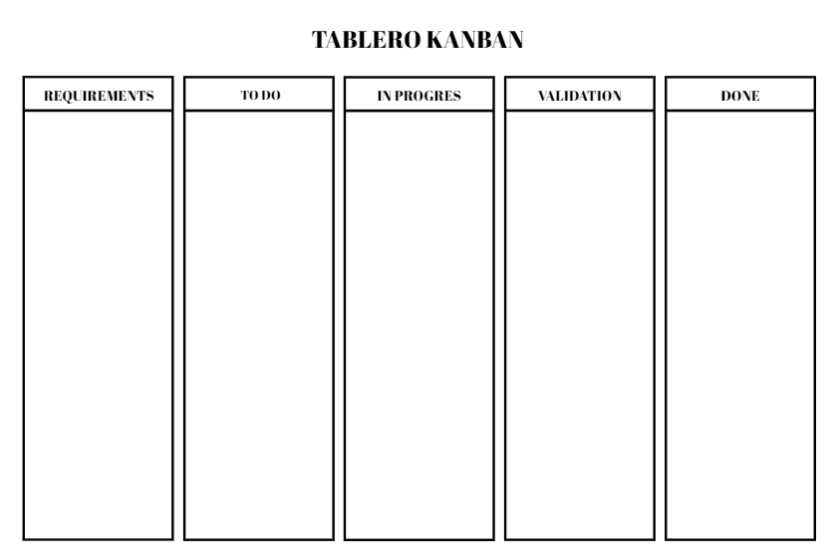
\includegraphics[width=0.5\linewidth]{tablero kanban validation}
\caption{Ejemplo con validación}
\label{fig:subrgrafo}
\end{figure}
	A continuación mostraremos como se ha utilizado y modificado el concepto de Tablero Kanban en este proyecto.\\
	Haremos la creación y seguimiento del tablero mediante Trello, un software de gestión de proyectos que mediante su interfaz de web permite fácilmente crear y customizar Tableros estilo Kanban. A continuación se muestra el tablero en un estado avanzado del desarrollo.\\
\begin{figure}[H]
\centering
  \centering
  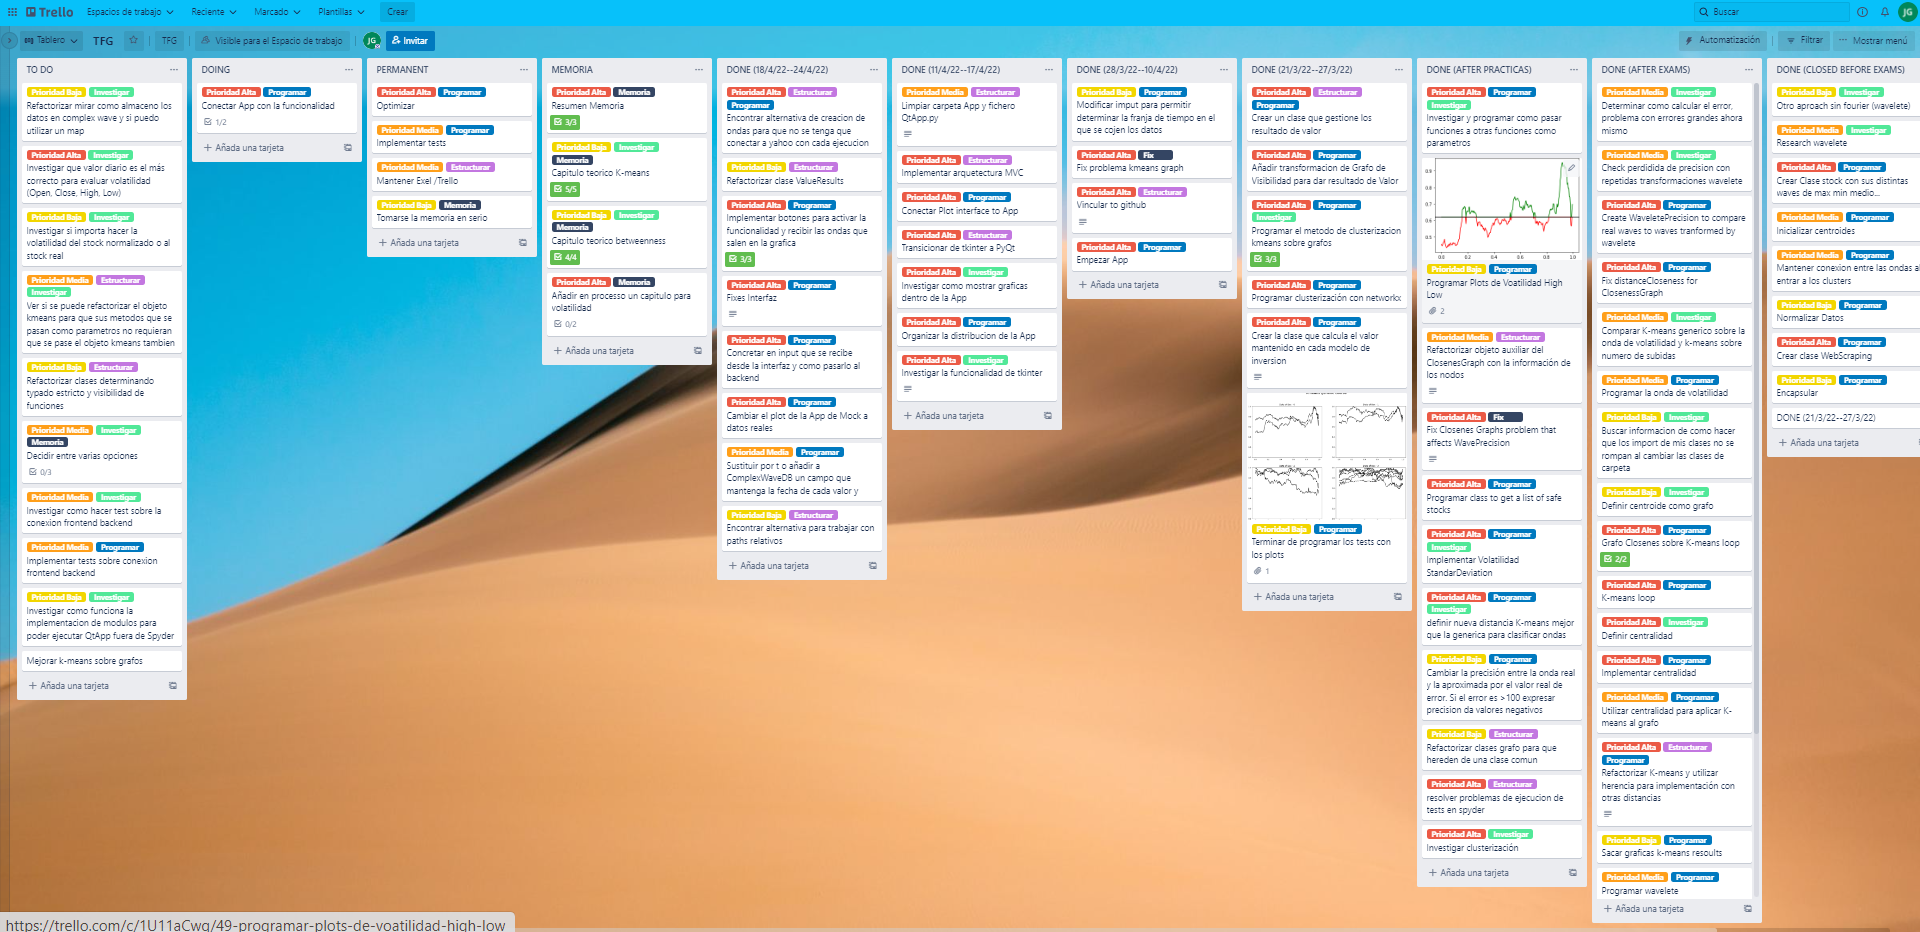
\includegraphics[width=1\linewidth]{trello}
\caption{Tablero usado en este proyecto}
\label{fig:subrgrafo}
\end{figure}
	Esta es una visión global del tablero por lo que es difícil ver todo lo que esta pasando, así que vamos a explicarlo parte por parte.\\
	\subsubsection{Nucleo}
\begin{figure}[H]
\centering
  \centering
  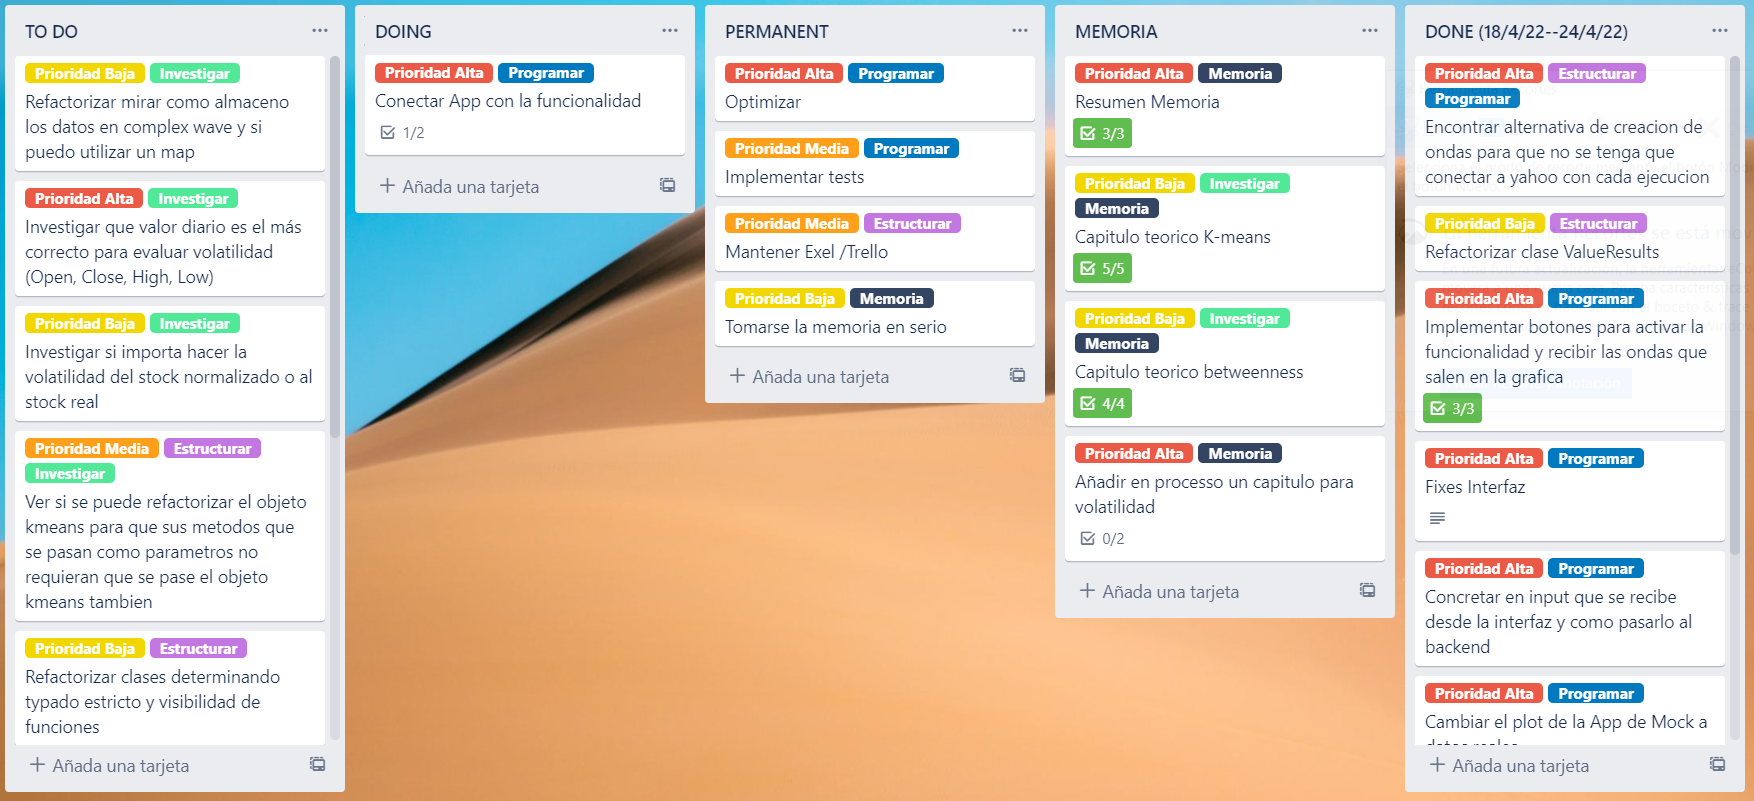
\includegraphics[width=1\linewidth]{trello nucle}
\caption{Nucleo del tablero Trello}
\label{fig:subrgrafo}
\end{figure}
	Esta es la parte principal del tablero y como podemos ver se parece mucho al esquema general, tenemos una columna TO DO con las tareas que no están empezadas, una columna DOING con las tareas en desarrollo.\\
	El cambio más notable de este tablero es la adición de una columna PERMANENT que aquí se utiliza para tener siempre en mente ciertas tareas, como puede ser "Implementar tests" para intentar maximizar la cobertura de los tests, o "Tomarse la memoria en serio" para recordar tomar notas durante el desarrollo del proyecto que ayude a la creación de la memoria.\\
	Por último tenemos dos tablas que tienen la misma razón de ser, tanto la columna MEMORIA como la columna DONE(18/4/22--24/4/22) se utilizan para almacenar las tareas que ya se han terminado, la diferencia es que en la columna DONE se almacenan las tareas que añaden valor al proyecto, y en la columna MEMORIA se guardan las tareas relacionadas con la creación de la memoria.
	\subsubsection{Tareas}

	Con las tareas nos referimos a cada uno de los items que se mueven a lo largo de las columnas de la tabla. Y por lo general lo que intentamos hacer con estas tareas es que cada una sea unitaria, es decir, que cada tarea pueda cumplir su funcionalidad sin necesidad de que las demás tareas cumplan la suya. Esto ademas nos permite testear la funcionalidad de cada tarea por separado sin depender de otras tareas.\\
	El problema es que estas tareas con los requisitos anteriores se nos pueden complicar mucho, o aumentar mucho de tamaño como podemos ver con el siguiente ejemplo de la tarea "Conectar App con la funcionalidad"\\
\begin{figure}[H]
\centering
  \centering
  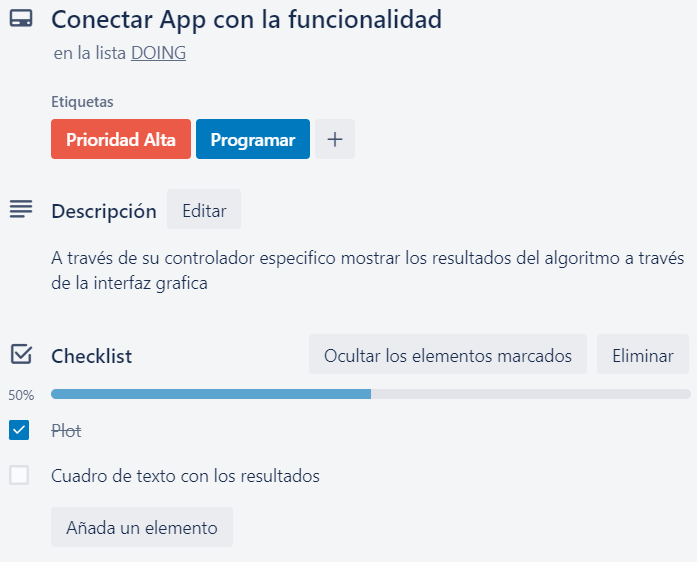
\includegraphics[width=1\linewidth]{trello tarea}
\caption{Ejemplo de tarea}
\label{fig:subrgrafo}
\end{figure}
	Esta tarea engloba todo el proceso de la salida de los datos por pantalla, y como hay dos formas de mostrar los datos en nuestra aplicación utilizamos un checklist para dividir esta tarea en subtareas, y cada unos de estas subtareas se encarga de conectar una parte distinta de la aplicación. Esto lo hacemos de este forma ya que Trello, a diferencia de otras herramientas como Jira, no permite la relación entre tareas, es decir, si creo as subtareas como items por si mismas no tengo forma de agruparlas bajo la misma funcionalidad.\\
	Además de esto, dentro de la tarea tenemos una pequeña descripción de la funcionalidad que se quiere implementar y tenemos asignadas a la tarea una serie de etiquetas, en este caso son "Prioridad Alta" y "Programar" que implican que la tarea conlleva tocar codigo, y que cuanto antes se termine mejor. Pero no solo existen esas etiquetas, a continuación mostramos todas las etiquetas que se han usado a lo largo del proyecto.\\
\begin{figure}[H]
\centering
  \centering
  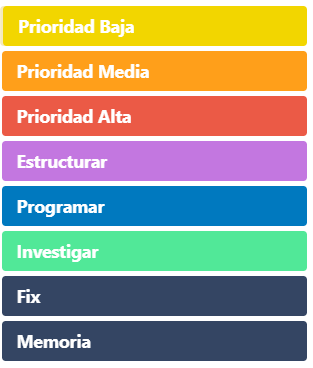
\includegraphics[width=0.5\linewidth]{trello etiquetas}
\caption{Repertorio de etiquetas usadas en este proyecto}
\label{fig:subrgrafo}
\end{figure}
	Las primeras etiquetas muestran la importancia de la tarea determinando grados de prioridad mientras que el resto de etiquetas muestran el dominio de la tarea.	\subsubsection{DONE}
\begin{figure}[H]
\centering
  \centering
  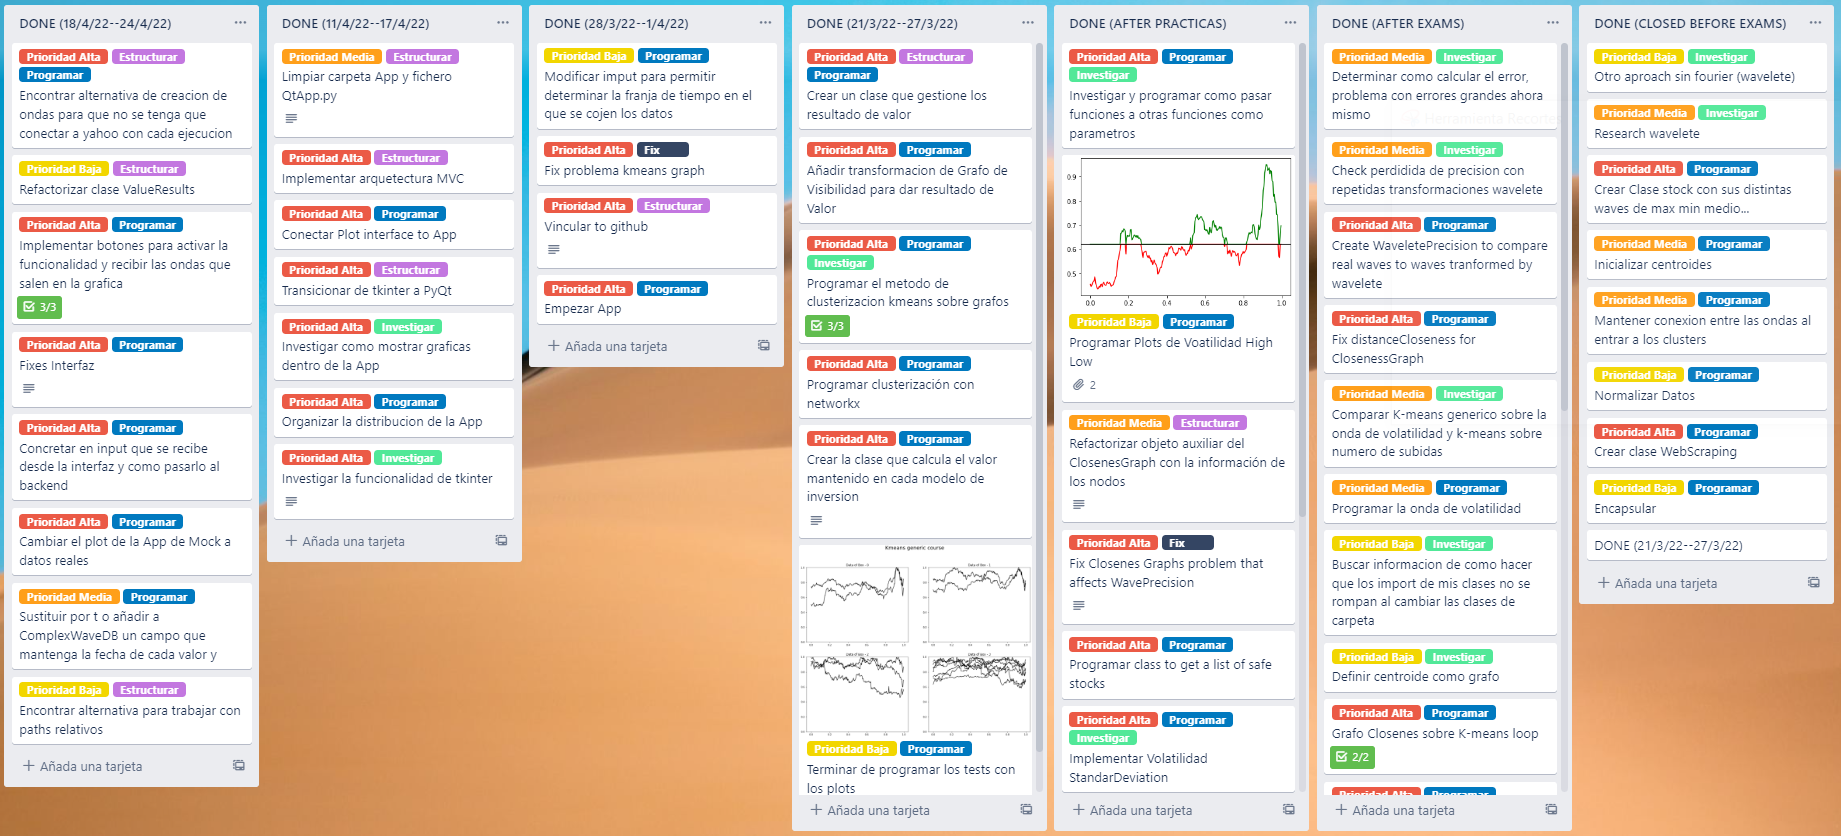
\includegraphics[width=1\linewidth]{trello done}
\caption{Archivo de las tareas realizadas}
\label{fig:subrgrafo}
\end{figure}
Aquí mostramos el resto del tablero, y como se puede ver consiste en todas las tareas que se han terminado repartidas dependiendo del intervalo de tiempo durante el cual se han completado. Esto, junto a un fichero Exel donde se ha apuntado el tiempo dedicado por día nos permite tener un buen esquema cronológico del desarrollo del proyecto.\\
Aquí mostramos un segmento del fichero Exel con estos datos, pero el fichero en su totalidad estará en los apéndices.\\
\begin{figure}[H]
\centering
  \centering
  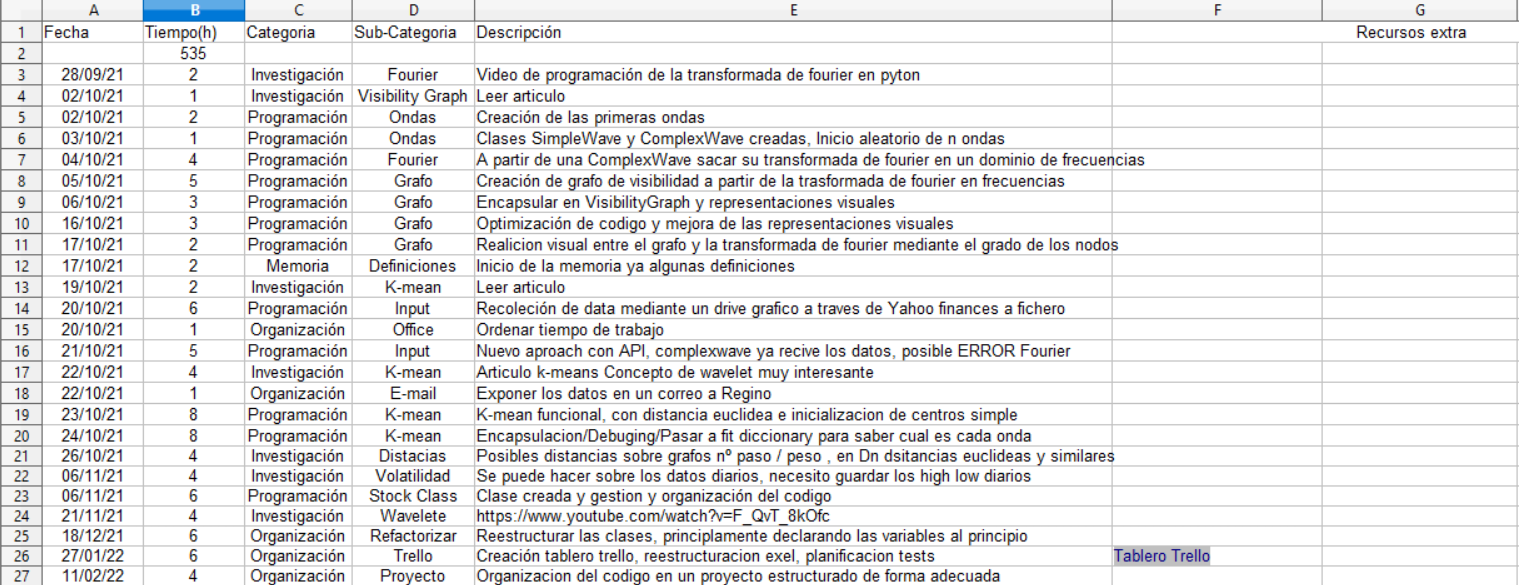
\includegraphics[width=1\linewidth]{exel}
\caption{Sección del documento Exel}
\label{fig:subrgrafo}
\end{figure}

	\subsection{Control de versiones}
	El concepto control de versiones se refiere a la gestión y almacenamiento de los distintos cambios que se hacen sobre un proyecto. Esto en la practica produce en registro de todas las versiones de un proyecto a lo largo del tiempo.\\
	Esto puede hacerse de varias maneras, la forma más rudimentaria que todo el mundo ha utilizado alguna vez es hacer el proceso de forma manual. Lo que consiste en duplicar los fichero del proyecto y guardarlos aparte, ya sea un USB, un disco externo, o el propio ordenador de trabajo. Esto se suele hacer como copia de seguridad del proyecto por si ocurre algo irreparable en el proyecto real, pero en cuando requerimos de mas instancias del proyecto guardadas nos topamos con problemas de organización y espacio muy rápidamente.\\
\begin{figure}[H]
\centering
  \centering
  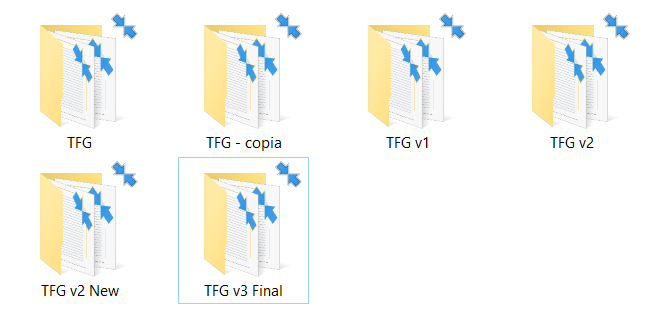
\includegraphics[width=1\linewidth]{control versiones mal}
\caption{Ejemplo de malas praxis de control de versiones}
\label{fig:subrgrafo}
\end{figure}
	Por esta razón es recomendable utilizar una herramienta de control de versiones que facilite la gestión de las instancias. Existen una gran cantidad de opciones pero nosotros hablaremos de una de las más populares, la cual es la que utilizaremos nosotros en este proyecto,esa herramienta es Git.\\
	Git permite alojar nuestro proyecto en un repositorio ajeno a nuestro ordenador lo que implica que el proyecto permanecerá seguro pase lo que pase con el ordenador desde el que se trabaja. El desarrollo del proyecto ocurre sobre una imagen local del proyecto que hay en el repositorio, y todo cambio que se quiera hacer permanente se tiene que subir al repositorio, a continuación mostramos como se hace ese proceso.\\
	Lo mínimo que tendríamos que hacer es:\\
	\begin{enumerate}
	\item \textbf{\$ git add .} para meter los cambios en el commit.\\
	\item \textbf{\$ git commit "Mensaje commit"} Efectuar el commit.\\
	\item \textbf{\$ git push} para pasar los cambios de local a remoto.\\
	\end{enumerate}
	
	Tan solo con proporcionarnos esta funcionalidad Git prueba que merece la pena ser utilizado, pero esto no es todo lo que puede hacer Git, ya que, bien utilizado Git permite la coordinación de equipos de desarrollo enteros sobre el mismo repositorio gracias a múltiples de sus herramientas, pero como este proyecto se ha desarrollado en solitario no nos meteremos en este tema. Es más, en el desarrollo de este proyecto ni siquiera vamos a utilizar Git por linea de comando ya que podemos instalar un plugin sobre Spyder que nos permite tener una pequeña interfaz mediante la cual gestionar la conexión con el repositorio Git como podemos ver a continuación.\\
\begin{figure}[H]
\centering
\begin{subfigure}{.5\textwidth}
  \centering
  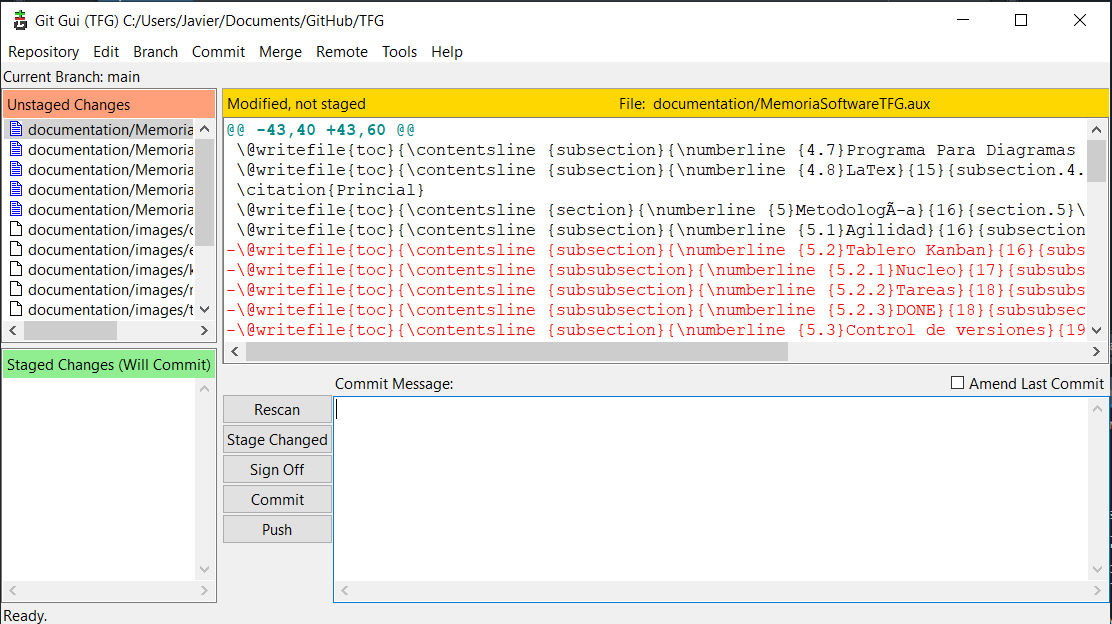
\includegraphics[width=.9\linewidth]{commit}
  \caption{Interfaz para realizar commit}
  \label{fig:sub1}
\end{subfigure}%
\begin{subfigure}{.5\textwidth}
  \centering
  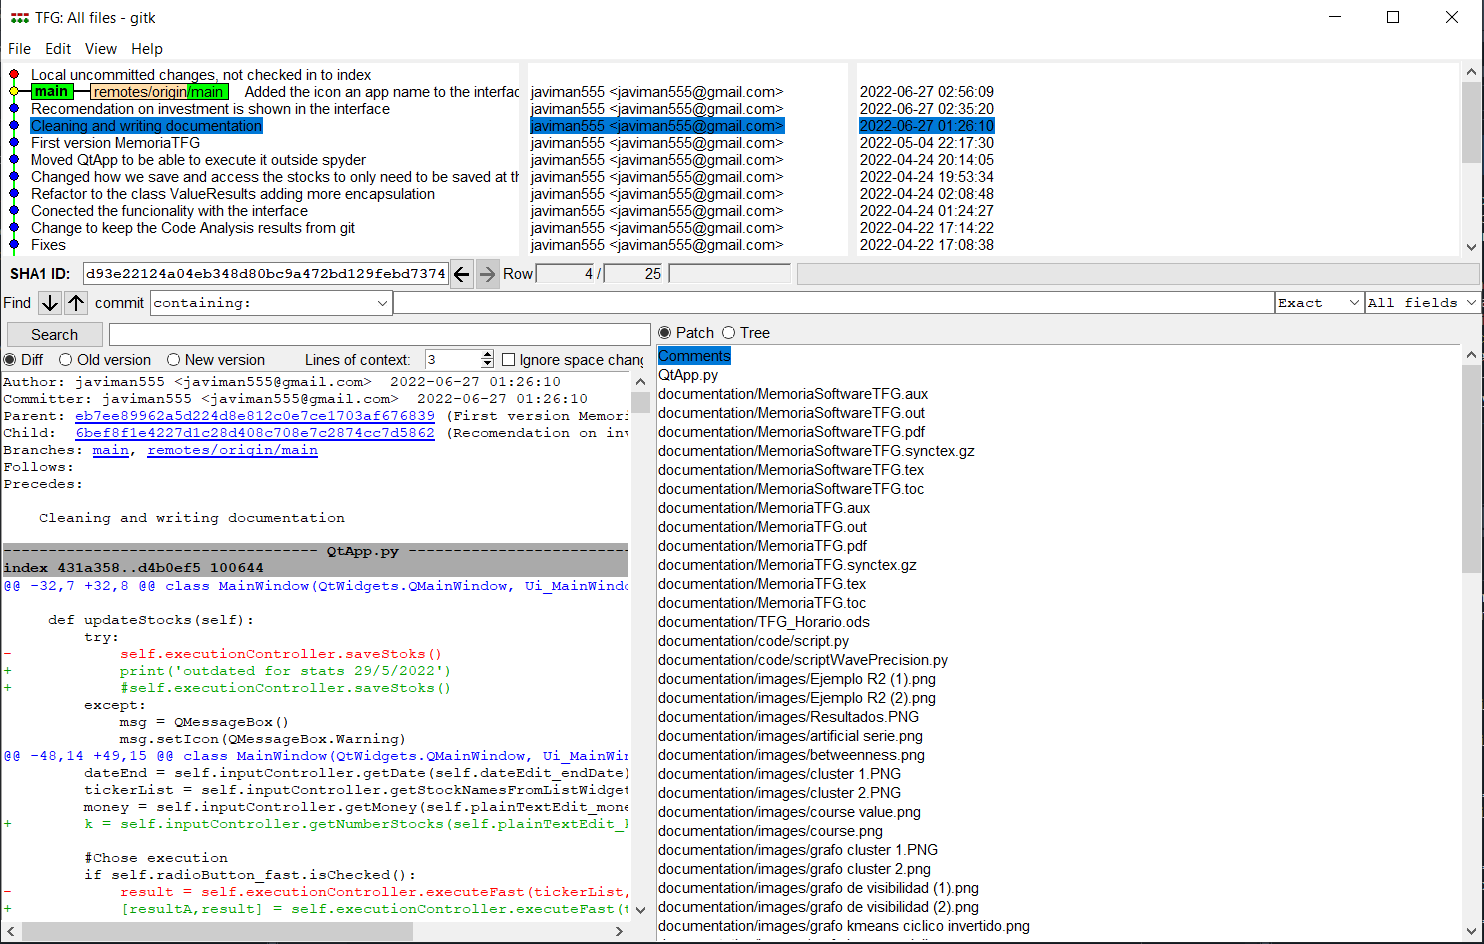
\includegraphics[width=.9\linewidth]{interface git}
  \caption{Interfaz del historial del repositorio}
  \label{fig:sub2}
\end{subfigure}
\label{fig:test}
\end{figure}
	Esta interfaz nos permite hacer los commits al repositorio de forma mucho más fácil, y hasta podemos ver el registro de cambios. Y todo lo que hagamos desde esta intefaz se ve reflejado en el repositorio. A continuación mostraremos el repositorio visto desde GitHub web para ver la similitud de las dos interfaces.\\
\begin{figure}[H]
\centering
  \centering
  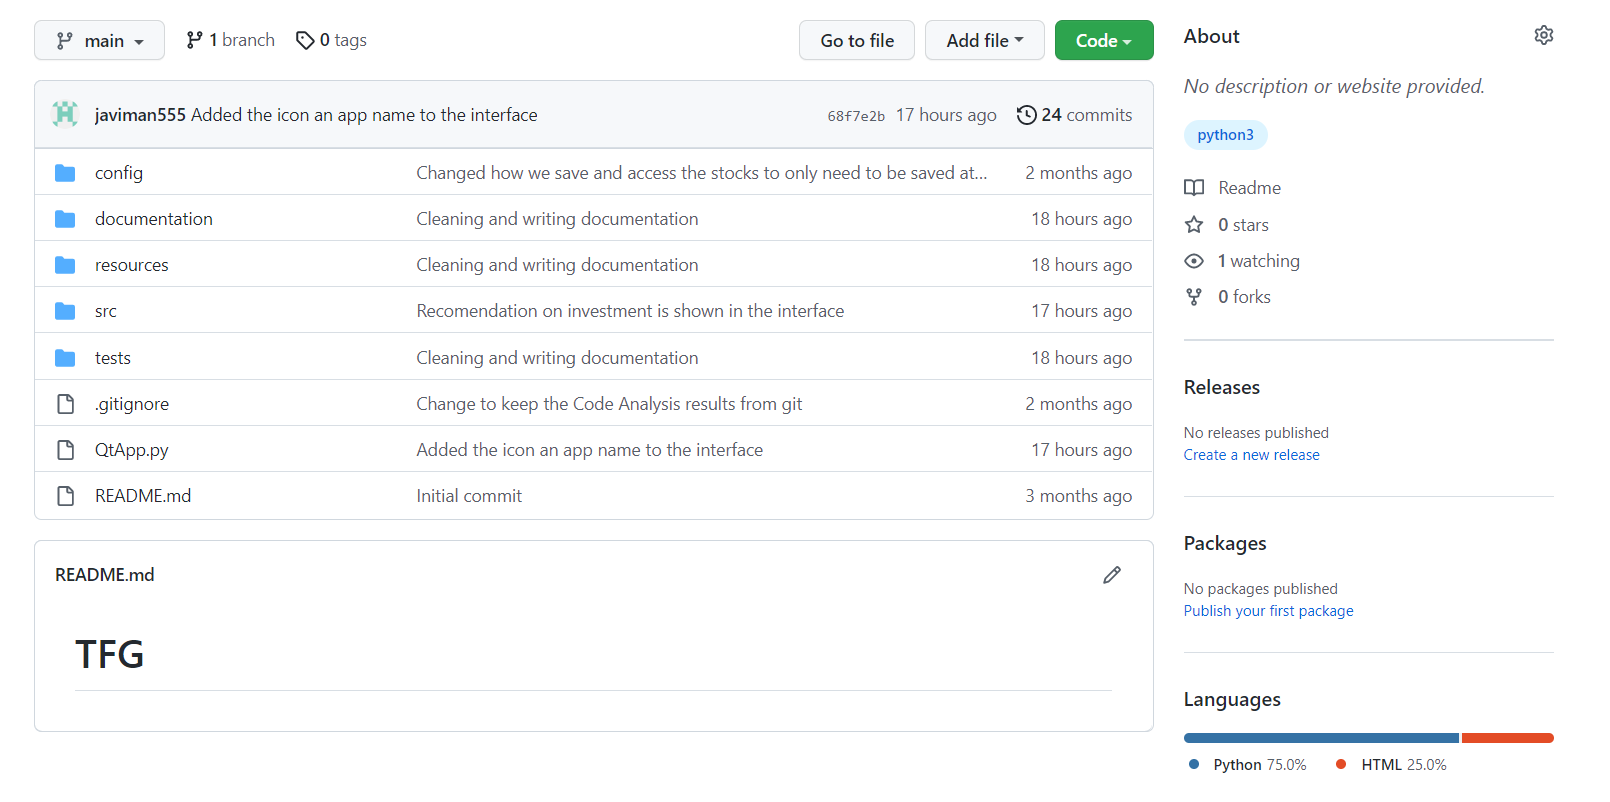
\includegraphics[width=1\linewidth]{github}
\caption{Repositorio desde web Github}
\label{fig:subrgrafo}
\end{figure}
	Se puede ver que GitHub web tiene una interfaz más refinada, pero la información del repositorio es la misma en ambas interfaces, y desde Spyder es mucho más fácil realizar los commits, por lo cual como no queremos instalarnos otra aplicación para realizar los commits como puede ser GitHub Desktop o Fork realizaremos los commits desde Spyder.\\
	Antes de terminar de hablar del control de versiones merece la pena mencionar que la implementación de Git en este proyecto se ha hecho bastante tarde ya que en un principio no se veía la utilidad, pero después de dos dolorosas sesiones de soluciones de errores que se alargaron más de la cuenta al romper partes del código que funcionaban como debían en los intentos de solucionar los errores se decidió añadir Git. En retrospectiva se debería haber usado Git desde el principio, pero por lo menos esto se tendrá en cuenta en proyectos futuros.\\
	
	
	\subsection{Tests}
	Antes de nada vamos a explicar a que nos referimos con tests y porque merece la pena implementarlos. Se conoce como test a un proceso automático que asegura el correcto comportamiento de una sección de código. Esto tiene una gran cantidad de ventajas muy importantes, como puede ser el proveer una detección de errores más rápida que la manual o el aislamiento del error al trozo de código que lo produce. Por lo general tener una baraja solida de tests es indispensable para el optimo desarrollo de un proyecto software, pero no nos podemos olvidar de que los tests consisten de más código que hay que mantener, así que es indispensable mantener los tests simples para limitar la carga técnica que se añade al proyecto. En la mayoría de los casos es mejor tener una mayor cantidad de test, los cuales individualmente son más simples, que tener muy pocos test muy complejos.
	En el desarrollo de este proyecto vamos a tener muy en cuenta los test para facilitar el desarrollo y sostenibilidad del proyecto, por eso vamos a implementar una practica de programación llamada TDD o Test-Driven Development (Desarrollo Dirigido por Tests) que nos ayudara a asegurar que los test cubran toda la funcionalidad del proyecto, nunca se podrá llegar a una cobertura del 100\%, pero esta practica ayuda a acercarnos a esa meta.\\
\begin{figure}[H]
\centering
  \centering
  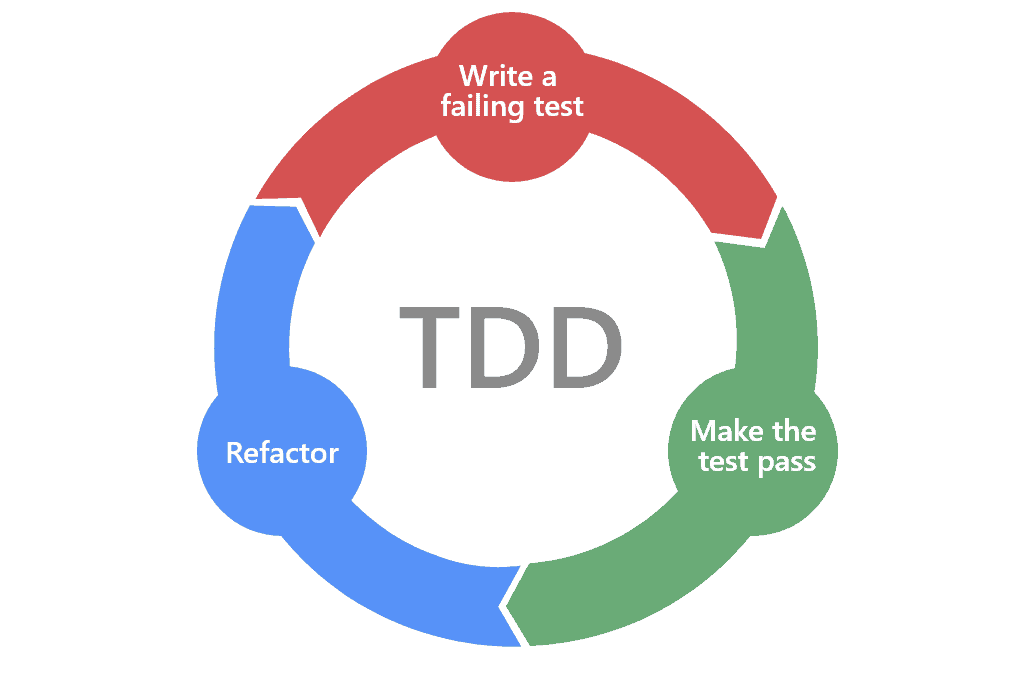
\includegraphics[width=0.5\linewidth]{test-driven-development-TDD}
\caption{Grafica TDD}
\label{fig:subrgrafo}
\end{figure}
	TDD tiene tres partes bien diferenciadas, y el proceso siempre es el mismo, para implementar cualquier cosa lo primero que se hace es escribir un test sobre la funcionalidad que se quiere implementar, obviamente el test falla porque todavía no hay nada implementado. El siguiente paso es implementar lo suficiente como para que el test deje de fallar, con esto se habría implementado dicha funcionalidad. Y ya lo que queda es refactorizar el código que hemos creado, haciendo que revisemos la implementación y aseguremos la calidad del código.\\
	 Hay una alta variedad de categorías de test como pueden ser:\\
	 \begin{enumerate}
	 \item \textbf{Tests Unitarios}: Suelen ser el nivel más bajo de test y comprueba en correcto comportamiento de métodos de clases de forma aislada.
	 \item \textbf{Tests de Integración}: Estos tests aseguran el correcto funcionamiento de las conexiones entre dos componentes distintos.
	 \item \textbf{Tests de Rendimiento}: Estos tests se centran en comprobar el rendimiento del código y evaluar la escalabilidad y fiabilidad del mismo
	 \end{enumerate}
	 Pero nosotros solo vamos a utilizar los tests unitarios ya que nuestro proyecto es lo suficientemente simple como para obviar los demás tipos de tests, siempre se pude en un futuro añadir otras clases de tests.\\
	 Los tests los implementaremos ayudándonos de otro plugin de Spyder llamado Spyder-unittest que provee las herramientas necesarias para una fácil creación de tests.\\

\begin{figure}[H]
\centering
\begin{subfigure}{.5\textwidth}
  \centering
  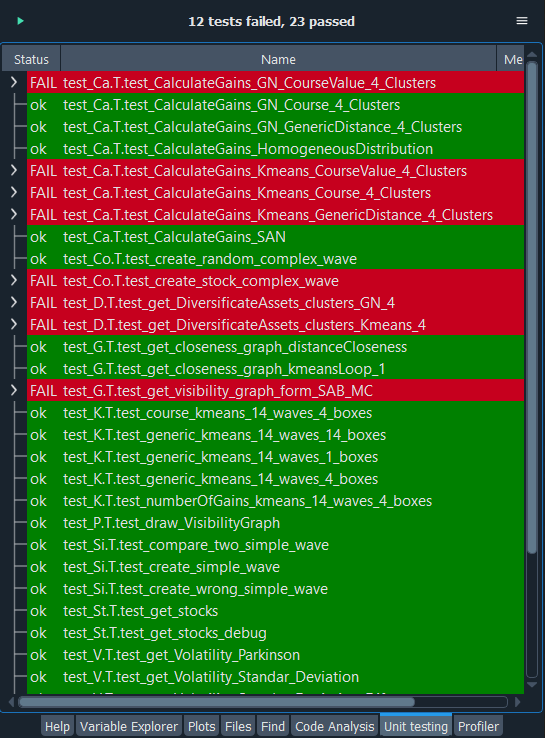
\includegraphics[width=.9\linewidth]{tests}
  \caption{Tests fallando}
  \label{fig:sub1}
\end{subfigure}%
\begin{subfigure}{.5\textwidth}
  \centering
  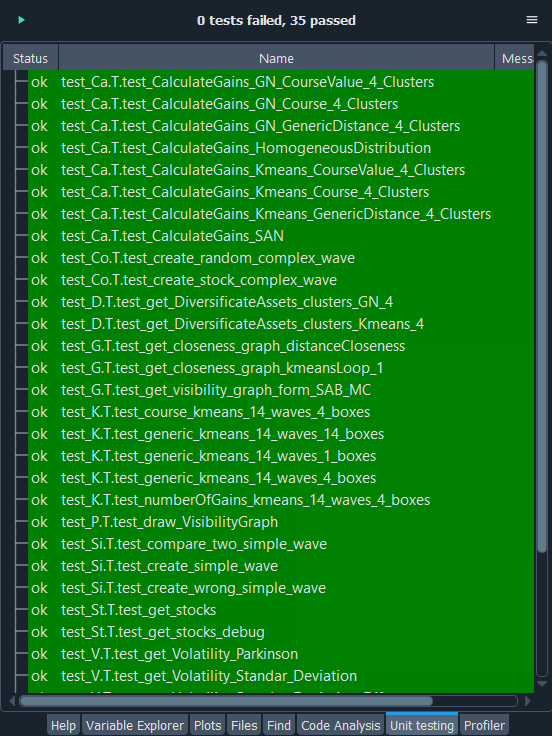
\includegraphics[width=.9\linewidth]{tests bien}
  \caption{Tests pasando}
  \label{fig:sub2}
\end{subfigure}
\label{fig:test}
\end{figure}
	 El uso de TDD se ha mantenido a lo largo de la mayor parte del desarrollo del proyecto, produciendo tests para la gran mayoría de clases funcionales del código, pero con la introducción de una interfaz en nuestro proyecto nos fue imposible mantener las pautas dadas por TDD como mostraremos a continuación.\\
	 
	\subsection{Interfaz}
	Se denomina interfaz a la conexión funcional entre dos sistemas o componentes que crea una vía para facilitar el intercambio de información. Para nosotros la conexión se efectúa entre el usuario y el programa mediante una interfaz gráfica muy simple como podemos ver a continuación.\\
	\begin{figure}[H]
\centering
  \centering
  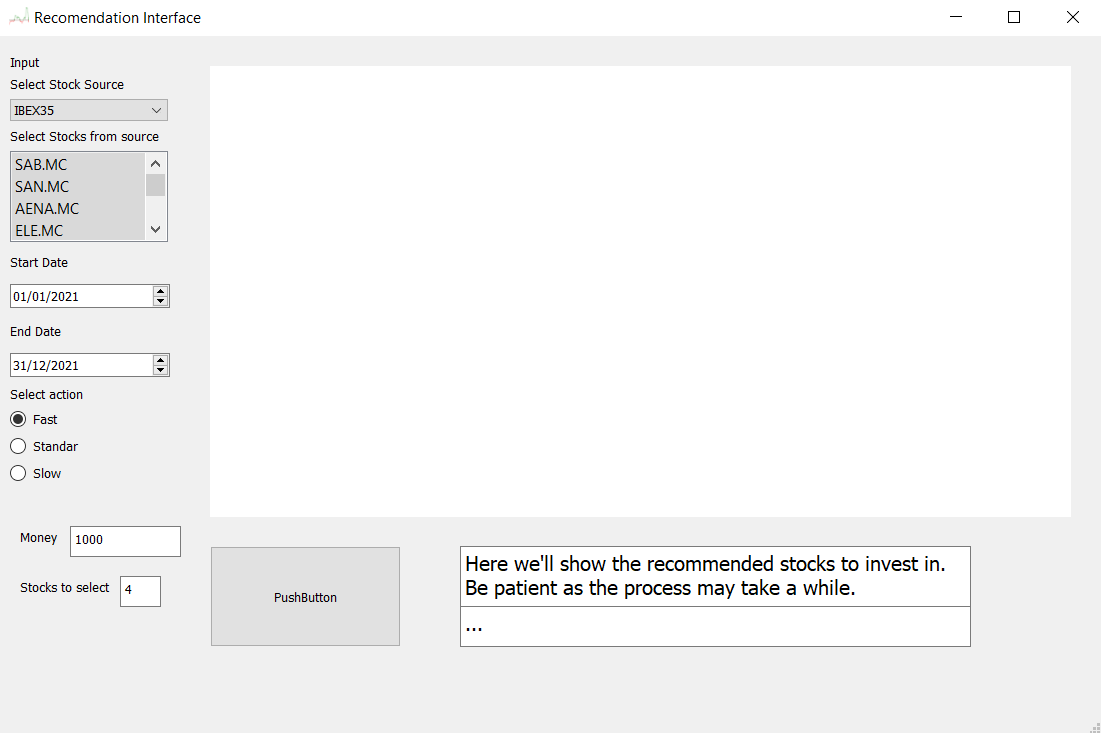
\includegraphics[width=1\linewidth]{interface}
\caption{Imagen interfaz gráfica de la aplicación}
\label{fig:subrgrafo}
\end{figure}
	 Esto permite al usuario interactuar de forma intuitiva con el programa.\\
	 Para desarrollar esta interfaz hemos buscado alternativas simples para crear aplicaciones pyton, y de esto forma a lo primero que llegamos fue a la librería gráfica \textbf{tkinter} ya que en su momento parecía la opción más simple, pero a lo largo del desarrollo de la aplicación se empezaron a ver sus limitaciones,la más relevante entre ellas es que tkinter no permite trabajar con htmls que es el formato en el cual generamos las gráficas con los resultados, por lo que en este punto hay que hacerse la pregunta,¿ modificamos el formato de las gráficas para poder seguir trabajando con tkinter o buscamos otra alternativa para hacer la interfaz gráfica?. Lo más fácil habría sido modificar el formato de las gráficas, pero en mi opinión esto es una mala practica ya que estamos modificando una parte del código que funciona perfectamente para acomodarnos a las restricciones de la interfaz, por lo que vamos a intentar buscar otra alternativa para crear la interfaz gráfica.\\
	 La alternativa que encontramos es utilizar la librería gráfica  \textbf{PyQt5} que además tiene la ventaja de ser compatible con la aplicación Qt Designer, un entorno de desarrollo gráfico permite crear y modificar la interfaz visualmente.\\
\begin{figure}[H]
\centering
  \centering
  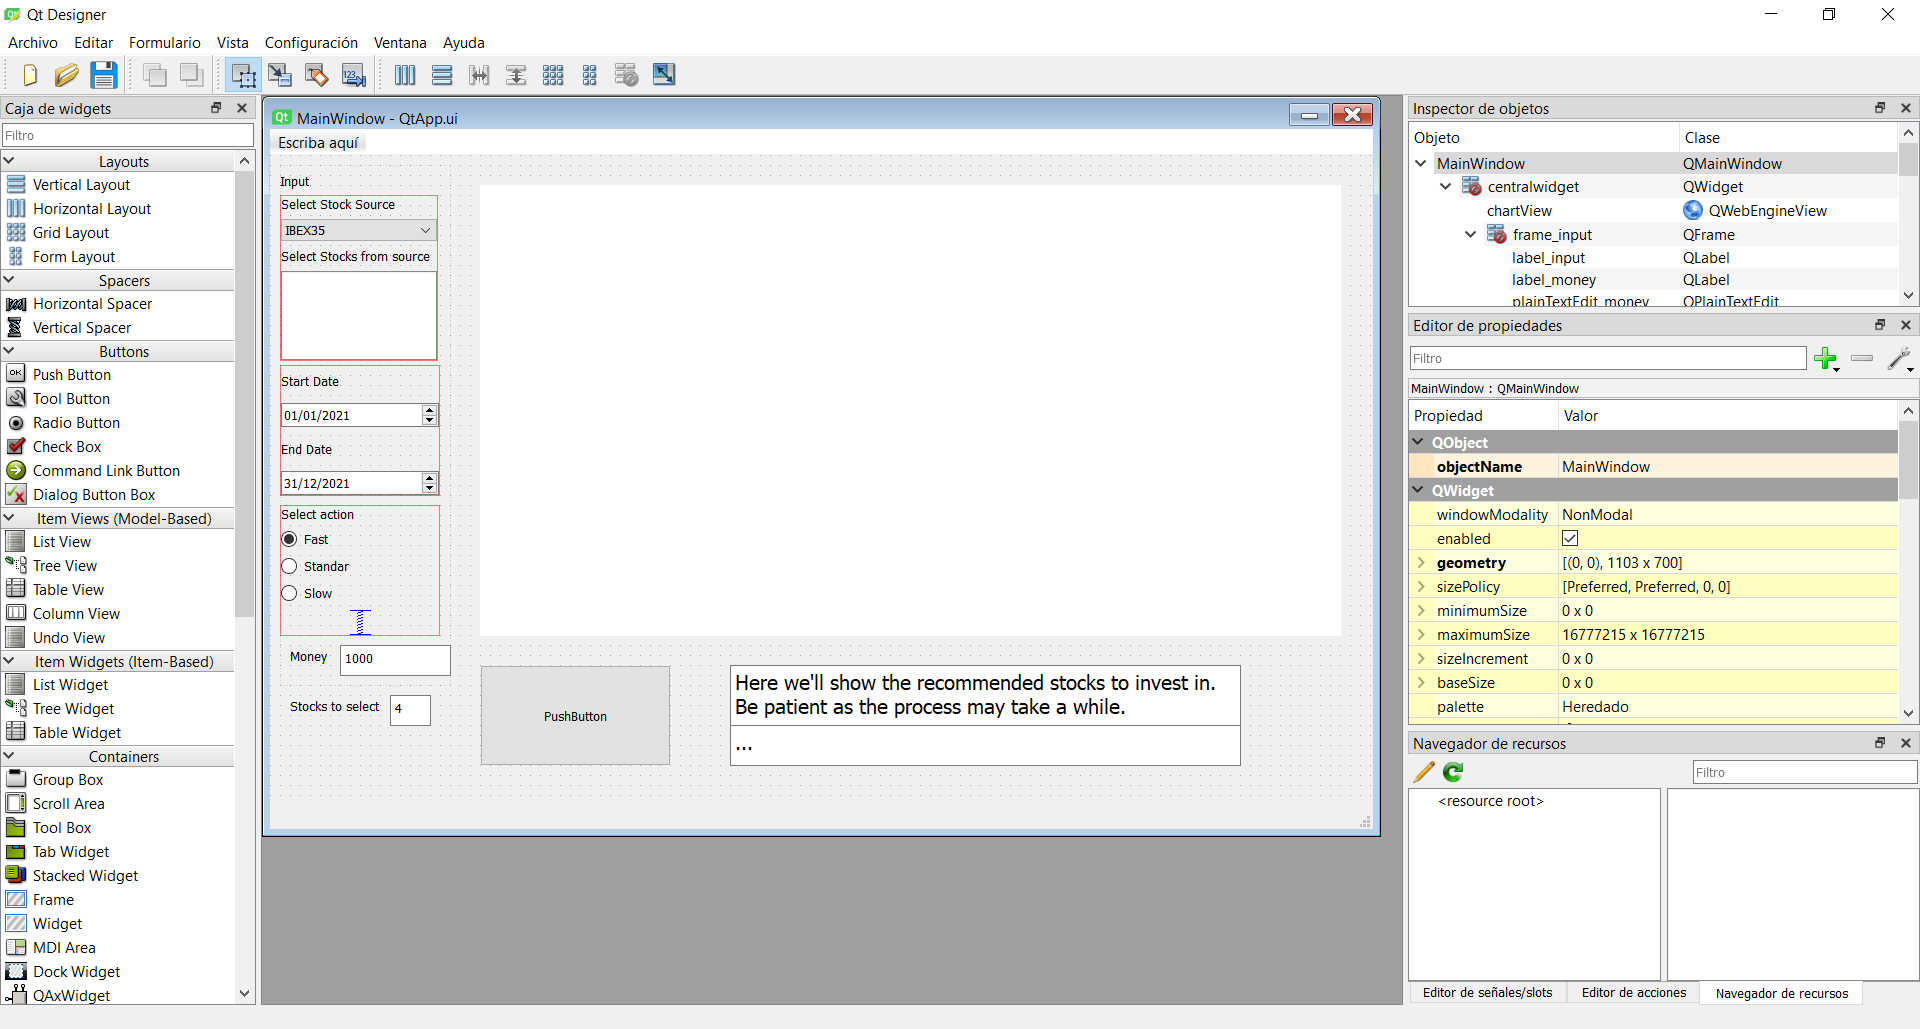
\includegraphics[width=1\linewidth]{qt designer}
\caption{Entorno de desarrollo Qt Designer}
\label{fig:subrgrafo}
\end{figure}

	 Con PyQt5 como alternativa a tkinter ya podemos migrar la interfaz a PyQt5, pero en este punto se hace aparente un fallo de diseño que hemos tenido hasta ahora. La conexión de la interfaz gráfica con la funcionalidad esta implementada de la siguiente forma:\\
\begin{figure}[H]
\centering
  \centering
  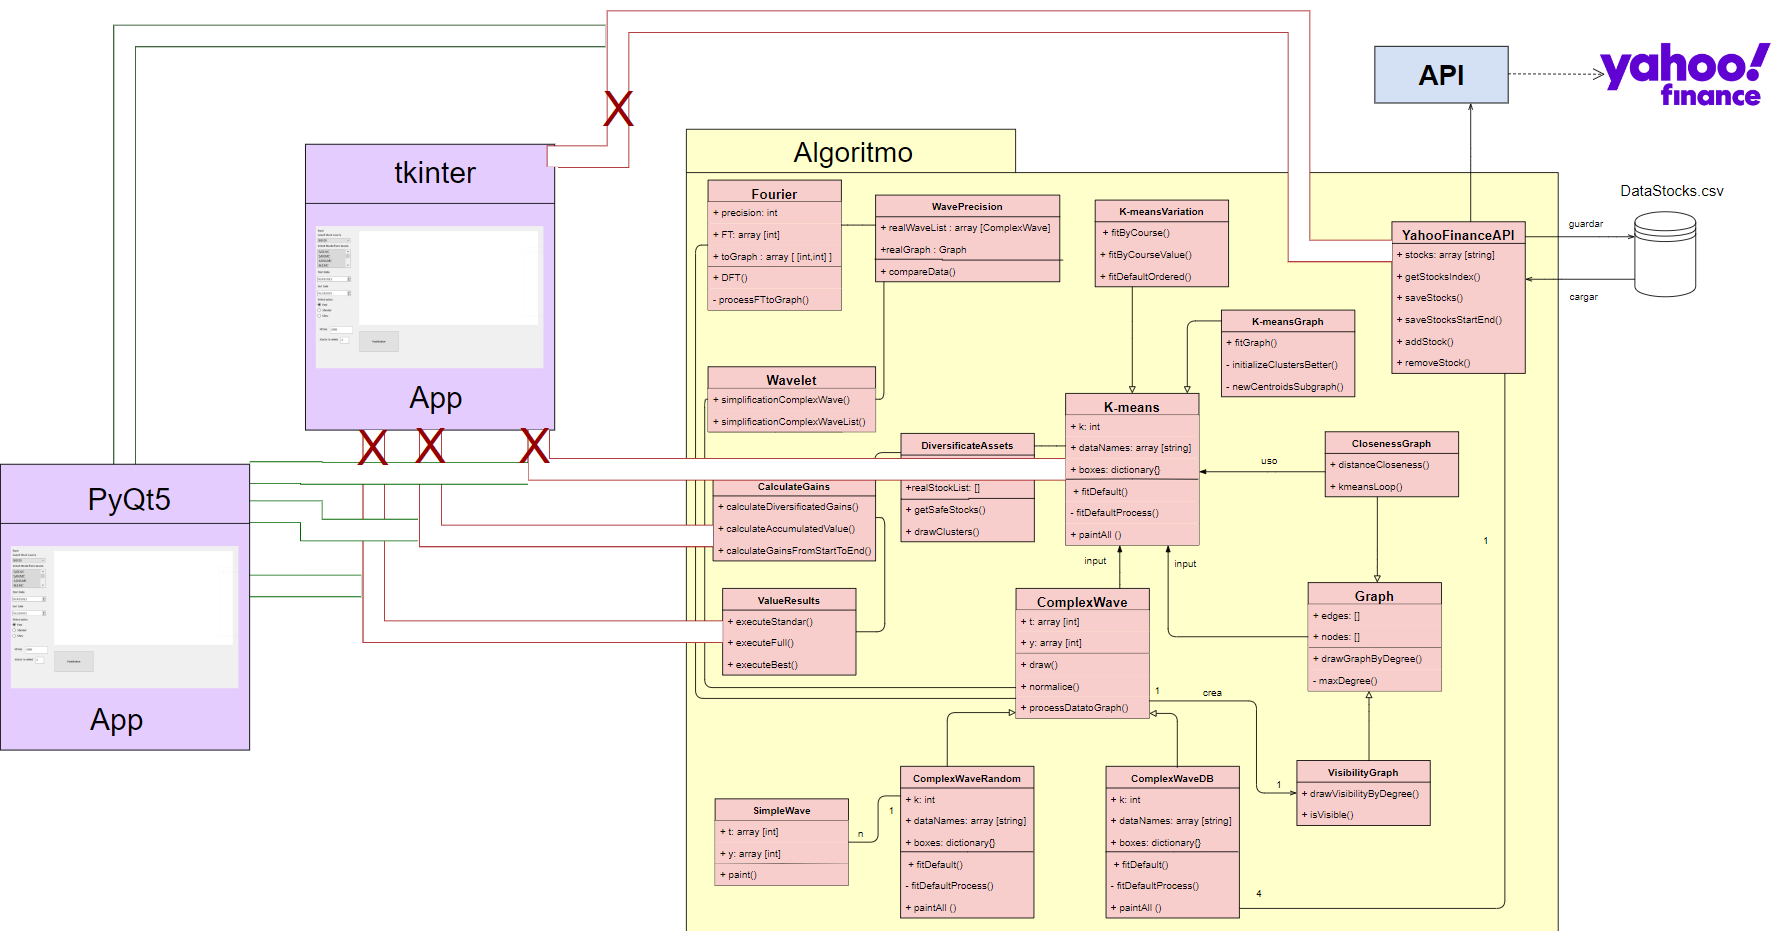
\includegraphics[width=1\linewidth]{Diagrama mal}
\label{fig:subrgrafo}
\end{figure}
	 Este diagrama muestra como la propia interfaz se comunica ella misma con cada una de las clases del procesos. Esto es un gran problema ya que ahora para migrar de interfaz hay que cambiar todas las conexiones haciendo que todo el código implementado para tkinter se tenga que desechar. Esto se podría haber solventado implementando una arquitectura modelo vista controlador, haciendo que la conexión entre la interfaz y la funcionalidad tenga esta pinta:\\
\begin{figure}[H]
\centering
  \centering
  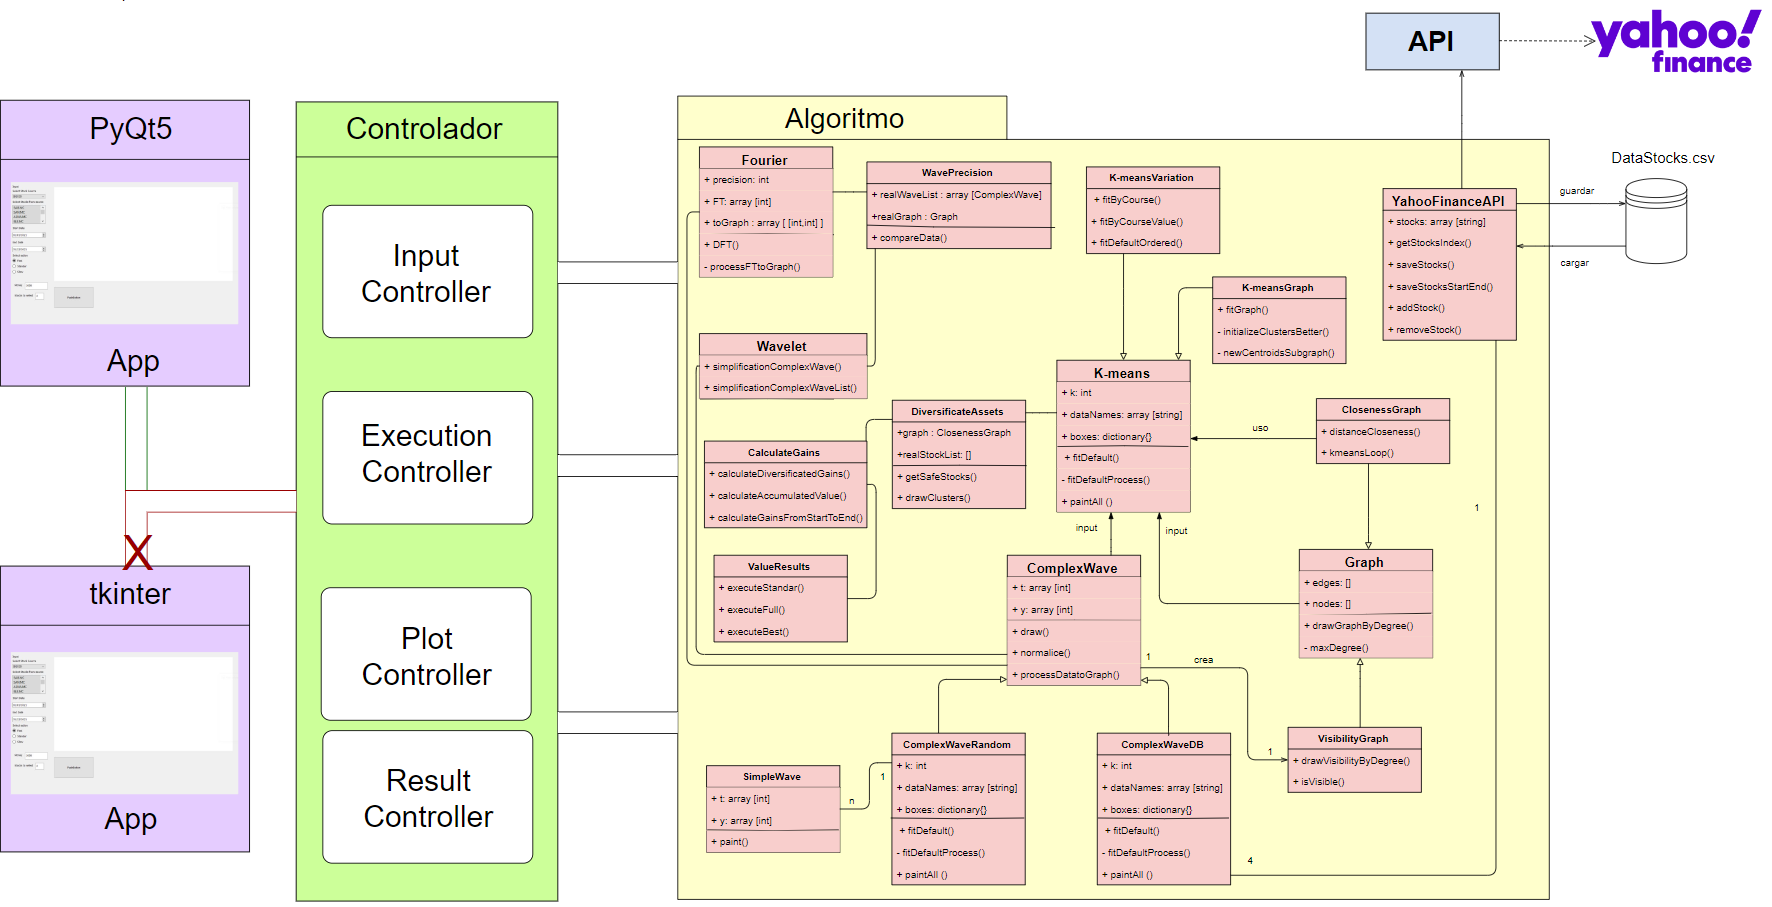
\includegraphics[width=1\linewidth]{Diagrama bien}
\label{fig:subrgrafo}
\end{figure}
	 Esto no se implementó antes debido al limitado tamaño del proyecto, pero en retrospectiva habría sido lo más adecuado, no solo por la migración de la interfaz sino también por los tests.\\
	 Cuando empezamos a desarrollar la interfaz nos topamos con el problema de que la librería de tests unitarios que utilizamos no estaba capacitada para tratar con la creación de aplicaciones, habríamos necesitado implementar un entorno de tests de integración, lo que nos resultaba demasiado complejo en ese punto. Por eso mismo violamos las pautas del TDD en este punto, pero ahora gracias a la decisión de diseño modelo vista controlador podemos testear la conexión entre la interfaz y la funcionalidad simplemente creando tests unitarios sobre los controladores. Por ejemplo, queremos testear que la selección de empresas en el frontend (Interfaz) queda reflejada en el backend, para esto solo necesitamos hacer un test unitario sobre el InputController.\\
	Así que podemos decir que gracias a implementar un diseño modelo vista controlador pudimos volver a cumplir las pautas del TDD.\\
\pagebreak

	\section{Arquitectura}
	\subsection{Fundamentos}
En un proyecto software consideramos que la arquitectura es el diseño de más alto nivel de la estructura del proyecto en cuestión. Para la creación de esta arquitectura se utilizan patrones de diseño y técnicas de abstracción que permiten al proyecto software realizar su función de la forma más optima. Con la función del sofware no nos referimos literalmente a que el software pueda realizar su función principal, eso es lo esperable con o sin una arquitectura bien definida, nos referimos a las funcionalidades secundarias del código como puede ser:
\begin{enumerate}
\item Sostenibilidad del código: Con esto nos referimos a la dificultad que reside en mantener el código del proyecto. Si el código es poco sostenible el coste, tanto económico como de complejidad, aumenta a lo lago del tiempo de forma descontrolada. Si el código es sostenible este aumento se pude reducir lo que en la practica extiende la vida útil del software.\\
\item Facilidad de expansión: Esto tiene que ver con el coste de implementar nueva funcionalidad a un código ya en producción.. A mayor facilidad de expansión menos aumenta el coste de cada sucesiva ampliación de funcionalidad, esto está ligado a la arquitectura del proyecto.
\item Seguridad: La seguridad de un software se refiere a la resistencia de dicho software a ataques. Estos ataques pueden ser de cualquier tipo, pueden ser intentos de acceso a información privada o ataques DDos(denegación de servicio) por mencionar algunos. Para prevenir estos ataques es necesario tener implementada una arquitectura segura.
\item Optimización de recursos: Este punto es el más fácil de explicar pero en la practica es sin duda uno de los más complejos. Simplemente consiste en minimizar los recursos, tanto de tiempo como de almacenamiento de datos, que se utilizar en la funcionalidad del proyecto.
\end{enumerate}
Dependiendo del tipo de proyecto en el que estemos se priorizaran de distinta forma estas metas. Por ejemplo si consideramos una aplicación de banca se prioriza la seguridad, pudiendo dejar en un segundo plano la optimización de recursos y eso se ve reflejado en la arquitectura del proyecto.\\
En nuestro caso priorizaremos la sostenibilidad del código y la facilidad de expansión sin tener muy en cuenta la seguridad ya que no trabajamos con ninguna clase de información delicada.\\
	\subsection{Modelo Vista Controlador}
	Ahora vamos a hablar de la mayor decisión arquitectónica que hemos implementado en este proyecto la arquitectura Modelo Vista Controladore (MVC), primero hablaremos en que consiste desde un punto de vista puramente teórico, y luego mostraremos como lo hemos implementado en el proyecto.\\
	La arquitectura MVC se centra en controlar el flujo de datos dentro del proyecto, define tres componentes distintos, Modelo, Vista y Controlador. Cada componente se ocupa de una tarea distinta y las conexiones entre los tres componentes están altamente restringidas.
	\begin{enumerate}
	\item El \textbf{Modelo} es lo que consideramos el backend del proyecto, es la parte del código que se encarga de toda la lógica del proceso, es decir, el acceso a los datos almacenados y el tratamiento de esos datos. Se puede considerar el núcleo del proceso y como tal suele tener la mayor parte de la complejidad computacional del proceso.
	\item La \textbf{Vista} se refiere a la interfaz de usuario y se encarga tanto de proveer un medio para mostrar información al usuario, como una ventana mediante la cual el usuario pueda interactuar con el proceso, lo podemos considerar el frontend de la aplicación.
	\item El \textbf{Controlador} es el intermediario entre el Modelo y la Vista, provee una vía para transportar los datos, y si es necesario transforma los datos para que el Modelo y la Vista se puedan entender. Es la parte del proceso más flexible, puede simplemente ser el link entra las otras dos capas, o puede ser el cerebro de la operación si se le añade un mínimo de lógica para que pueda controlar el flujo de la información.
	\end{enumerate}
\begin{figure}[H]
\centering
  \centering
  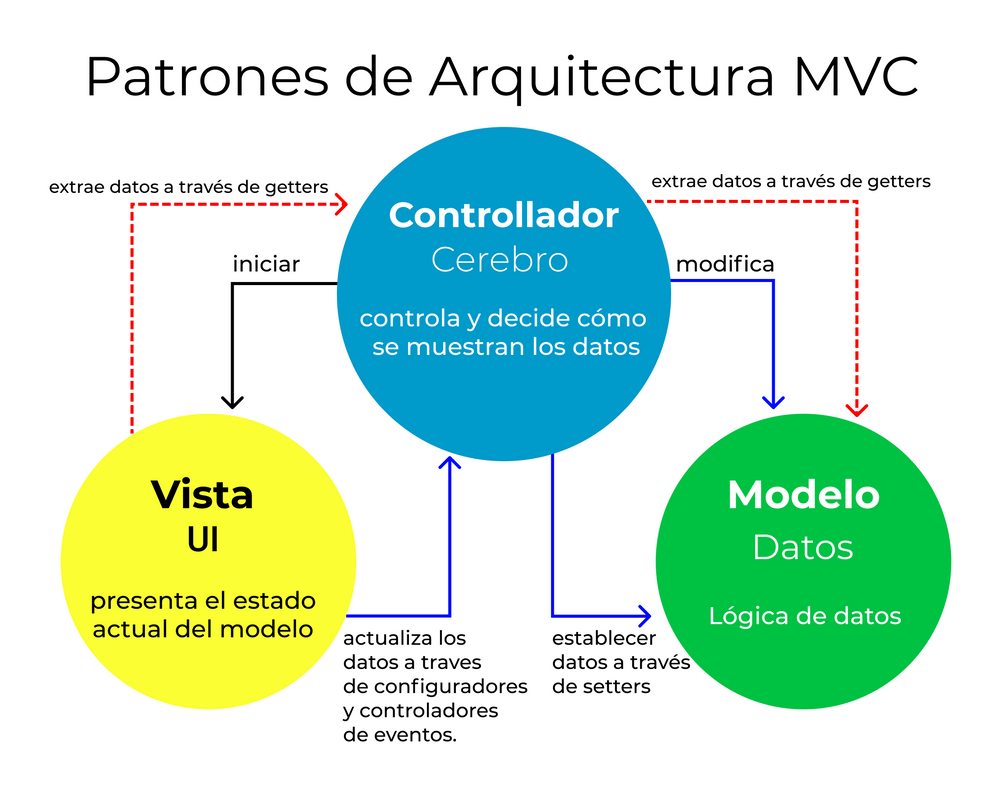
\includegraphics[width=1\linewidth]{MVC3}
\caption{Esquema Modelo / Vista / Controlador}
\label{fig:subrgrafo}
\end{figure}
	En nuestro proyecto tendremos la siguiente separación, mostrada intuitivamente en la organización de las carpetas del proyecto como podemos ver en los apéndices.\\
	Tenemos una carpeta con los controladores separados según la parte del proceso que gestionan, el InputController se encarga de recoger la información de entrada decidida por el usuario, el ExecutionController se encarga de llamar a la ejecución del programa, y tanto PlotController como ResultController se encargan de mostrar los resultados al usuario, por ultimo tenemos AltairPlot separado del PlotController por si en un futuro se quiere cambiar el tipo de plot que se muestra por pantalla de Altair a otro formato.\\
	Por otro lado tenemos la carpeta que contiene el modelo, en la cual nos meteremos más adelante, y por ultimo tenemos la vista, que tiene tanto la interfaz PyQt5 en QtApp\_ ui.py con su esquema en QtApp.ui como la antigua interfaz tkinter en App\_ Old.py.\\
	\subsection{Estructura de Modelo}
	Dentro del modelo tenemos la estructura de carpetas que se ve en los apéndices,\\
	No vamos a meternos todavía en la funcionalidad especifica de cada clase, lo que si que vamos a hacer es representar las conexiones mediante el siguiente diagrama.\\
\begin{figure}[H]
\centering
  \centering
  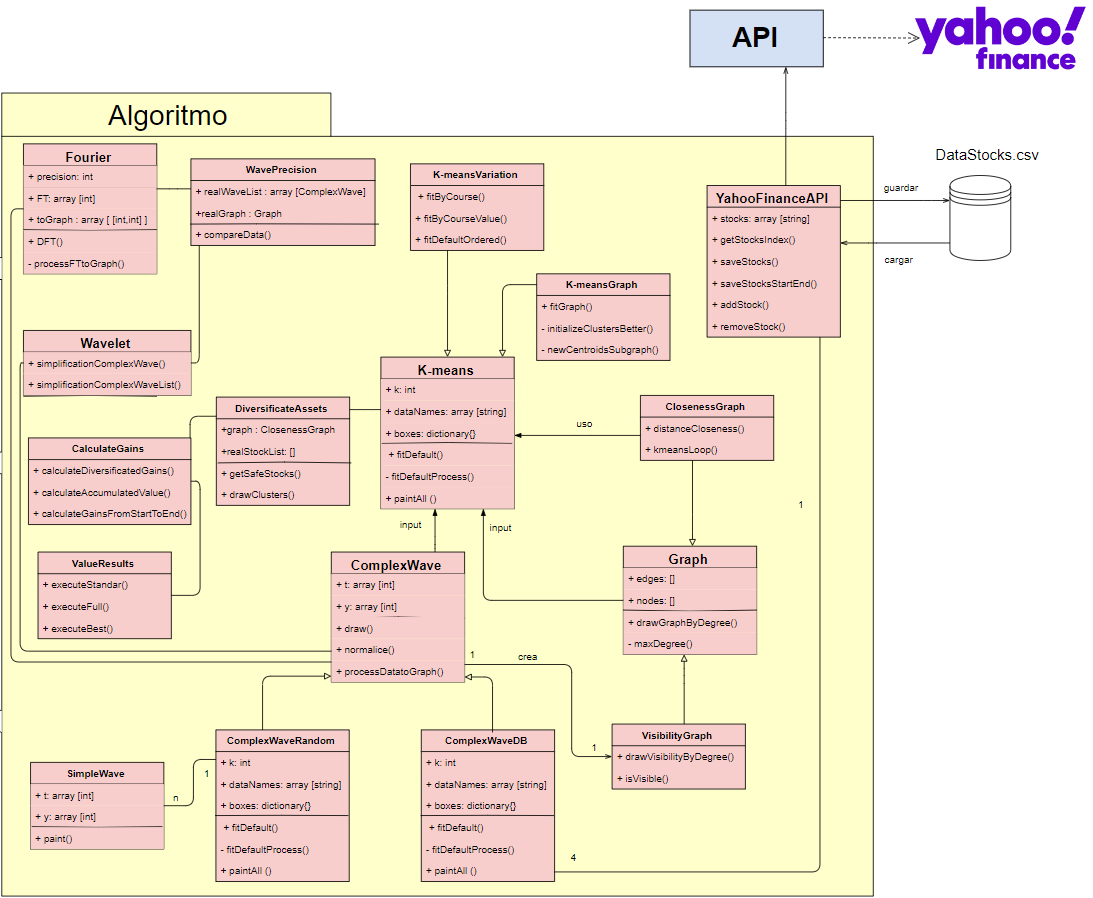
\includegraphics[width=1\linewidth]{Diagrama clases}
\caption{Diagrama de clases del modelo}
\label{fig:subrgrafo}
\end{figure}
	\subsection{Estructura completa}
	Con el núcleo del programa ya explicado podemos dar un paso atrás y ver la estructura global del proyecto como vemos en los apéndices.\\
	Ahora explicaremos cada uno de los elemento que tenemos.\\
	\begin{enumerate}
	\item \textbf{config}: Aquí se guardan las variables universales de todo el código, como son el día actual o la ruta del proyecto.
	\item \textbf{documentation}: Aquí se guardan todos los ficheros informativos del proyecto. Por un lado tenemos los fichero utilizados para hacer las memorias del proyecto,los ficheros TEX que generan las memorias en PDF,los recursos utilizados en estas memorias y los propios PDFs. Y por el otro lado tenemos un par de ficheros donde se han ido tomando apuntes a lo largo del desarrollo del proyecto como son Bibliografia.txt y TFG\_ Horario.ods.
	\item \textbf{resources}: Esta carpeta contiene los recursos que utiliza o genera el proyecto. En data están los ficheros csv que hacen el papel de base de datos del proyecto, en graphs tenemos todos los gráficos que hemos generado en el desarrollo de este proyecto, output contiene los resultados que hemos utilizado para el estudio presente en \cite{Princial} y App.ico es el icono de la interfaz gráfica.
	\item \textbf{src}: Aquí esta el código del proyecto que ya hemos mencionado antes.
	\item \textbf{tests}: Aquí tenemos todos los tests que se han ido creando a lo largo del desarrollo, todos estos tests son unitarios y cada fichero se encarga de testear la clase que indica su nombre.
	\item \textbf{Otros ficheros}: Por ultimo tenemos el fichero ejecutable QtApp.py que nos abre la interfaz gráfica de la aplicación y el README.md que contiene un resumen del proyecto.
	\end{enumerate}
	En conjunto esto nos crea la siguiente estructura de proyecto:\\
\begin{figure}[H]
\centering
  \centering
  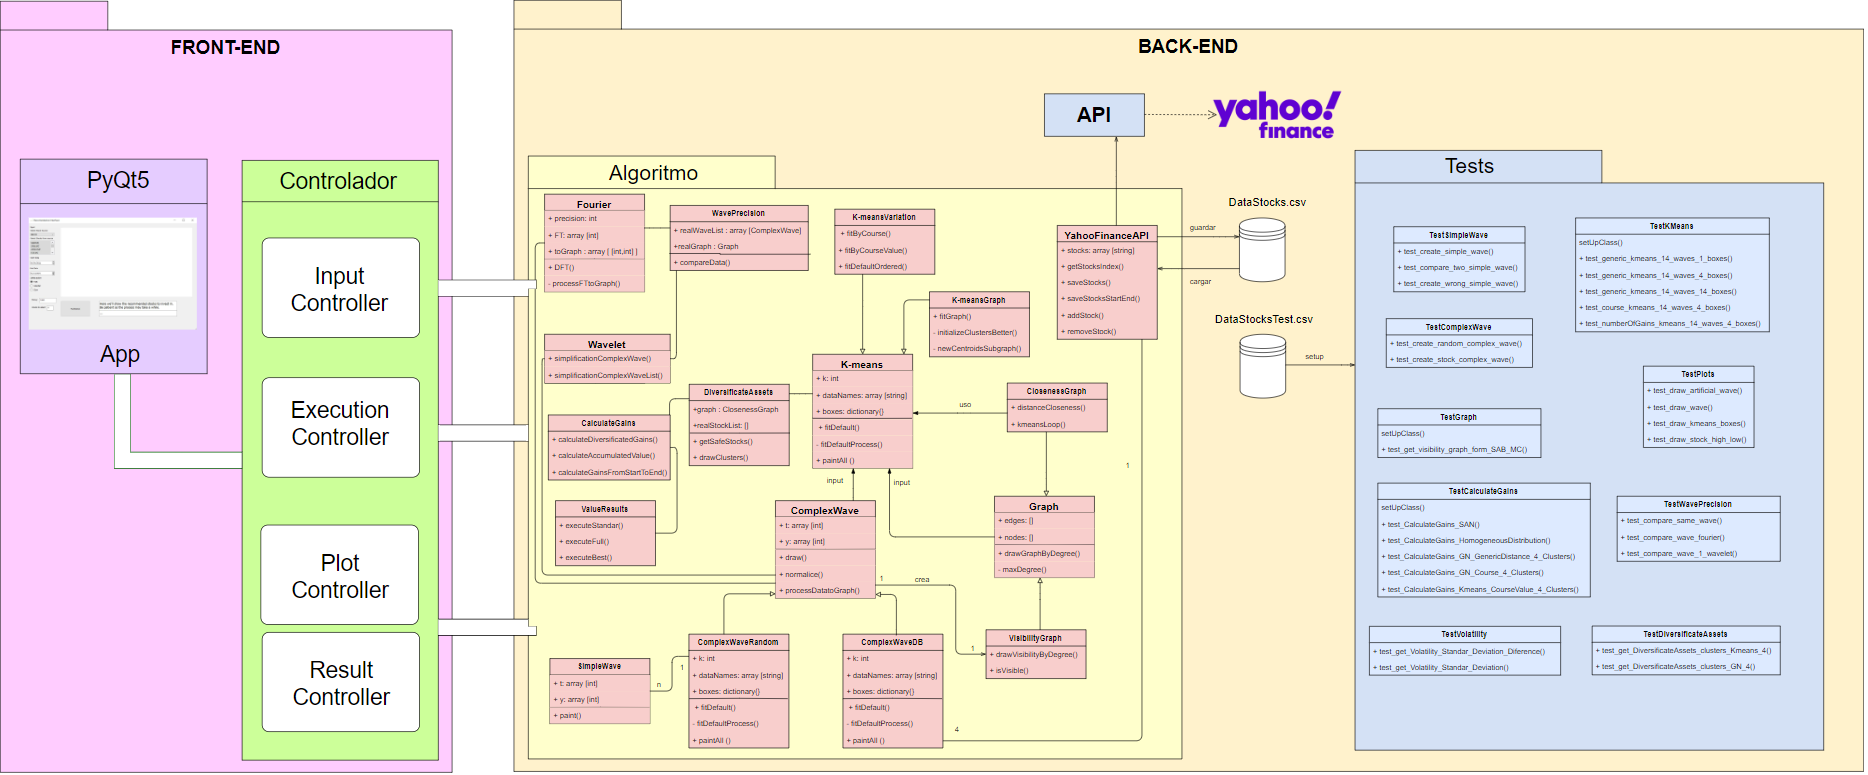
\includegraphics[width=1\linewidth]{Diagrama proyecto completo}
\caption{Diagrama de componentes del todo el proyecto}
\label{fig:subrgrafo}
\end{figure}
	La información más importante que recordar de este diagrama es que los tests y el modelo acceden a datos distintos, esto es un punto muy importante ya que permite el total desacoplamiento de los tests.


\pagebreak

	\section{Desarrollo}
	Con la estructura explicada podemos empezar a hablar del desarrollo en sí. Vamos a dividir el desarrollo en 3 etapas las cuales son fácilmente diferenciables debido a notables mejoras en la gestión del trabajo a lo largo del tiempo.\\
	\begin{enumerate}
	\item \textbf{Fase 1}: Etapa inicial en la que para documentar y gestionar el proyecto tan solo se utilizó un documento Exel para tomar notas.
	\item \textbf{Fase 2}: Etapa intermedia en la que se mejoró la gestión de las tareas añadiendo un tablero Trello.
	\item \textbf{Fase 3}: Ultima etapa en la que por fin se añade un sistema real de control de versiones como es Git.
	\end{enumerate}
	\subsection{Fase 1 (Exel)}
	Aquí tenemos documentado todo lo que se hizo en esta fase:\\
\begin{figure}[H]
\centering
  \centering
  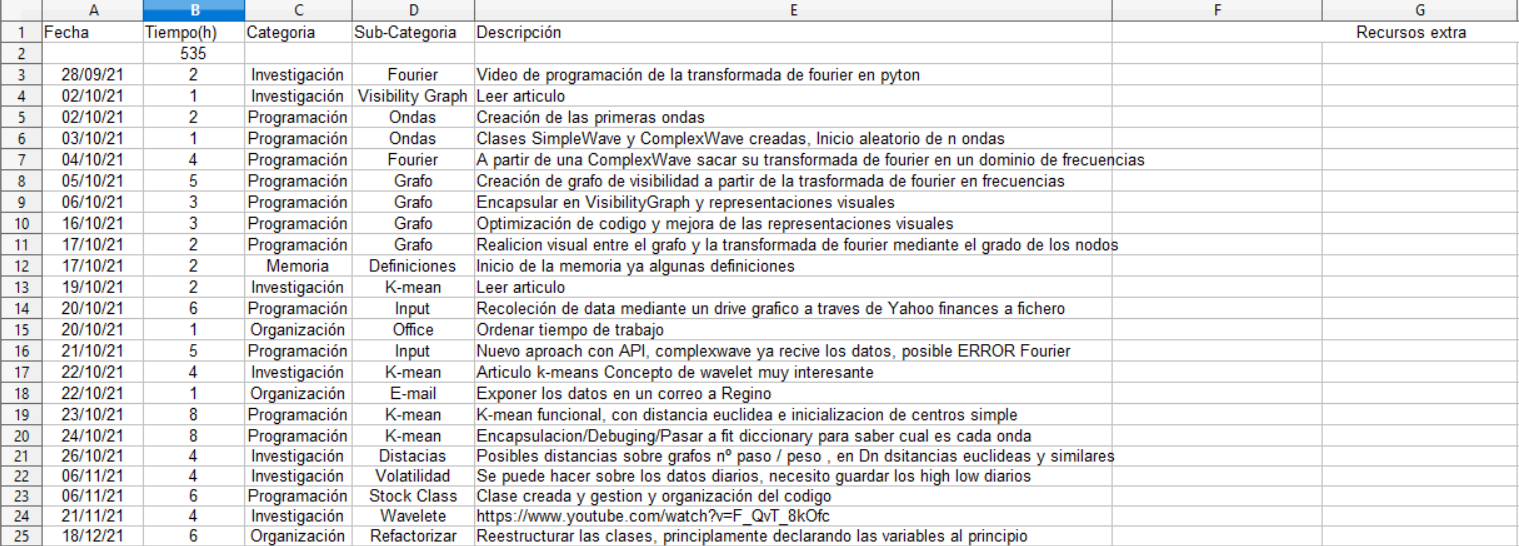
\includegraphics[width=1\linewidth]{exel fase 1}
\label{fig:subrgrafo}
\end{figure}
	Engloba un periodo de 3 meses en los cuales se realizan unas 84 horas de trabajo distribuidas de la siguiente forma:\\
	\begin{figure}[H]
\centering
  \centering
  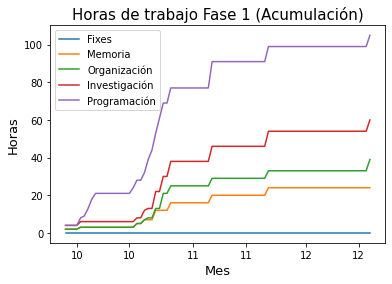
\includegraphics[width=0.5\linewidth]{tiempo fase 1}
\label{fig:subrgrafo}
\end{figure}
	La mayor parte del tiempo es utilizado programando, en este punto se crean las primeras versiones de los objetos que utilizaremos en el algoritmo.Estos objetos son SimpleWave y ComplexWave que son los primeros objetos que contienen la serie temporal que se le pasa al algoritmo como input. También tenemos las transformaciones que se aplicaran a las series temporales como son Fourier, Wavelet y VisibilityeGraph. Y se importa el algoritmo K-means sin modificar en la clase K-mean que servirá de base para nuestro algoritmo. Por ultimo se crea una vía para recoger datos de stocks que se convertirán en series temporales.\\
	
	La estructura del proyecto es la siguiente al final de esta fase:\\
\begin{figure}[H]
\centering
  \centering
  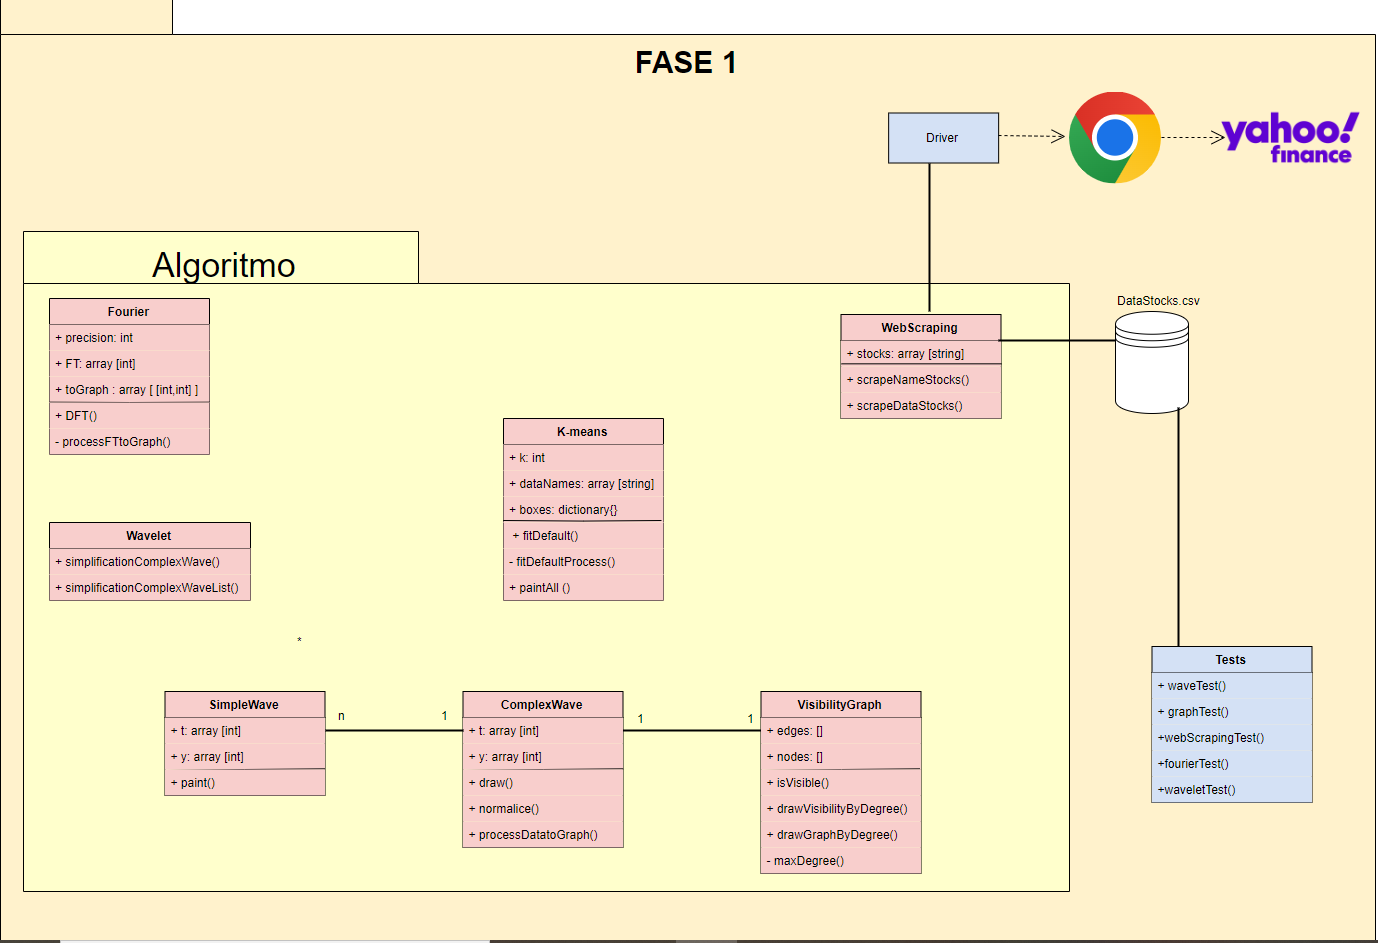
\includegraphics[width=1\linewidth]{Fase 1}
\label{fig:subrgrafo}
\end{figure}
	Lo más relevante es que en este punto los tests están acoplados al resto del código, esto se debe principalmente a que aunque hemos estado siguiendo un desarrollo TDD, no hemos utilizado herramientas que facilitan la creación y uso de los tests como puede ser el plugin unittest de Spyder que utilizaremos en las siguientes fases. Esto quiere decir que los tests han sido más costosos de crear, y lo que es todavía más relevante, los tests han tenido que ser ejecutados a mano uno a uno hasta ahora.\\ 
	Por otro lado podemos ver que las clases todavía no estas conectadas entre ellas.\\
	\subsection{Fase 2 (Trello)}
		Aquí ya tenemos implementado el tablero Trello para gestionar las tareas a realizar:\\
\begin{figure}[H]
\centering
  \centering
  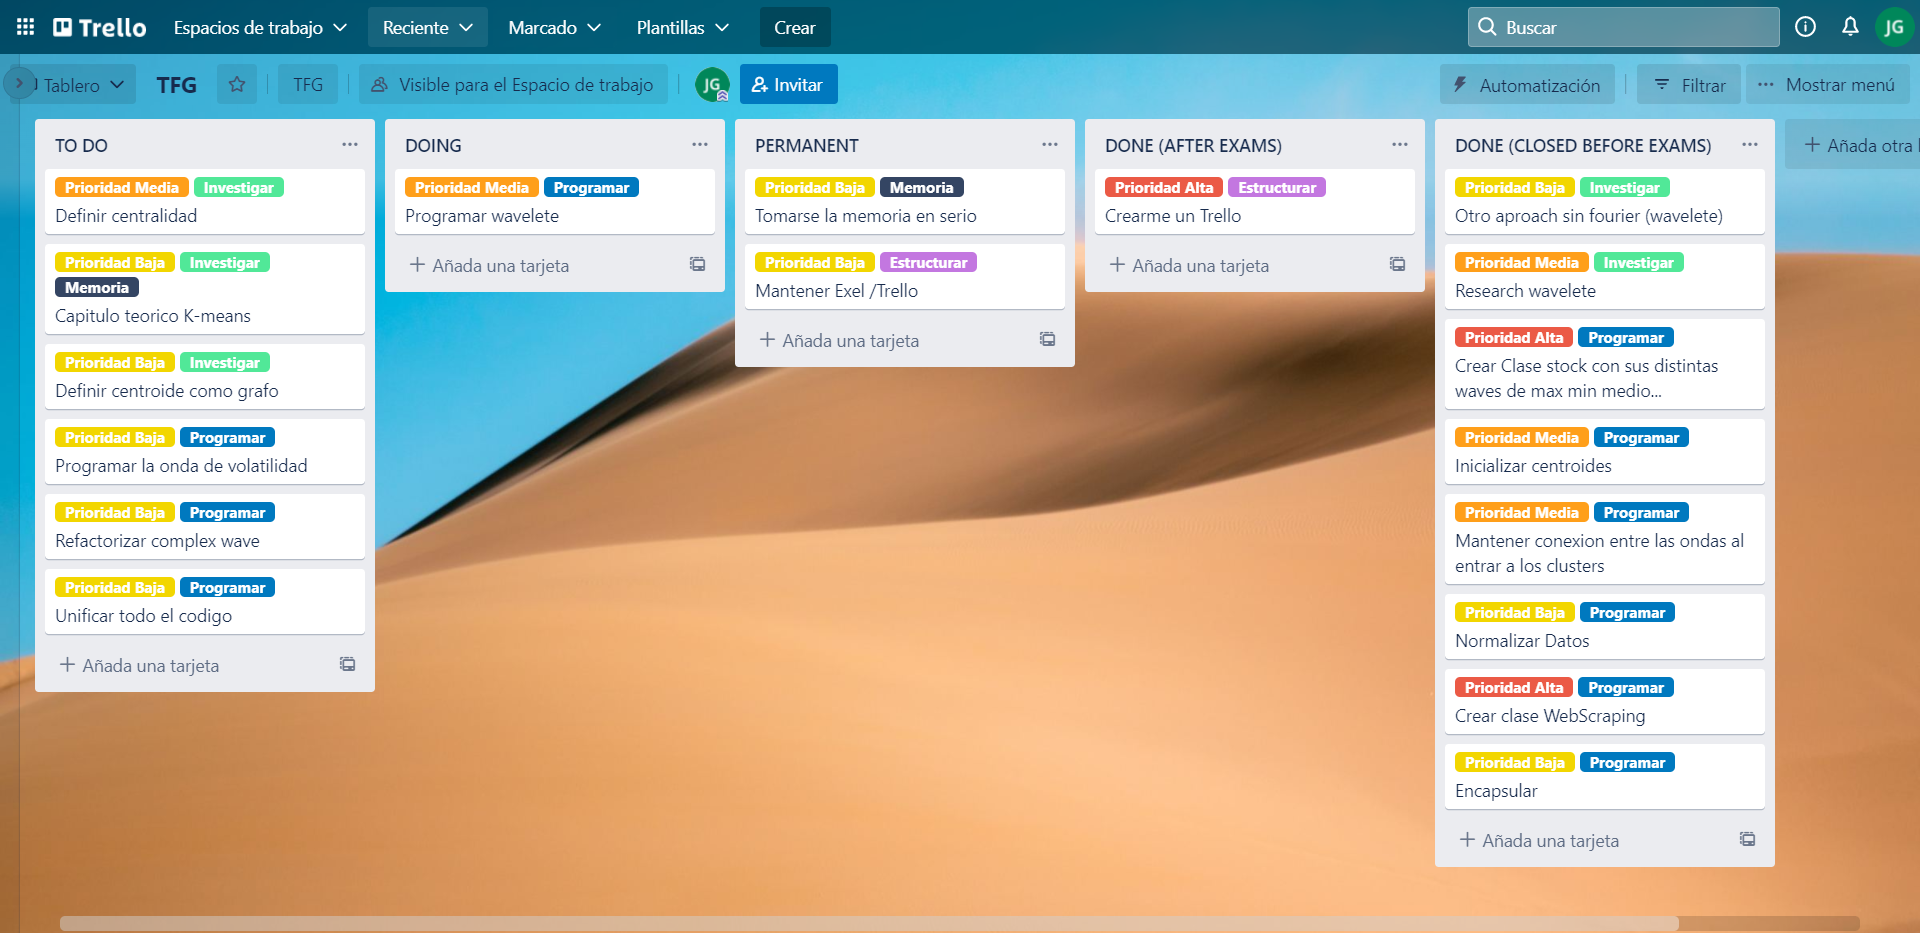
\includegraphics[width=1\linewidth]{Tablero Trello Creado}
\label{fig:subrgrafo}
\end{figure}
	Engloba un periodo de 3 meses en los cuales se realizan unas 272,5 horas de trabajo distribuidas de la siguiente forma:\\
\begin{figure}[H]
\centering
  \centering
  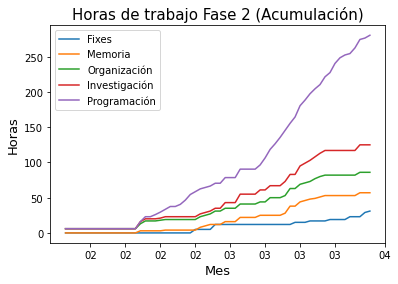
\includegraphics[width=0.5\linewidth]{tiempo fase 2}
\label{fig:subrgrafo}
\end{figure}
	\textbf{Grafica de tiempo Fase 2}\\
	En esta fase seguimos manteniendo que la mayor parte del tiempo se ha usado programando, lo cual no es extraño ya que en esta fase completamos la funcionalidad del algoritmo en su totalidad.\\
	Lo primero que hacemos es implementar herencia sobre ComplexWave, Graph y K-mean lo que nos permite generalizar la funcionalidad de estos objetos, todavía no hemos desacoplado los tests.\\
\begin{figure}[H]
\centering
  \centering
  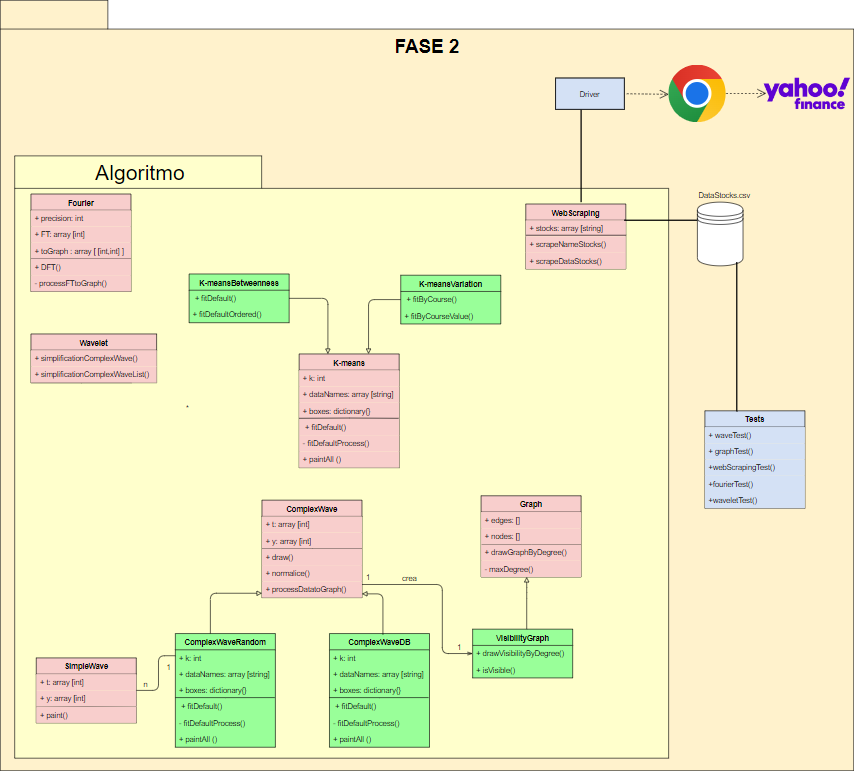
\includegraphics[width=1\linewidth]{fase 2 herencia}
\label{fig:subrgrafo}
\end{figure}
	Luego desarrollamos pequeñas customizaciones sobre K-means sirviéndonos de que acabamos de implementar herencia, y conectamos las clases para tener la primera versión funcional del algoritmo. Un punto muy importante es que desechamos la primera idea de recolección de data a través de un driver que hace de automata ante un cliente chrome, ya que es absurdamente complejo en comparación con la alternativa de utilizar una API a yahoo finances\\
\begin{figure}[H]
\centering
  \centering
  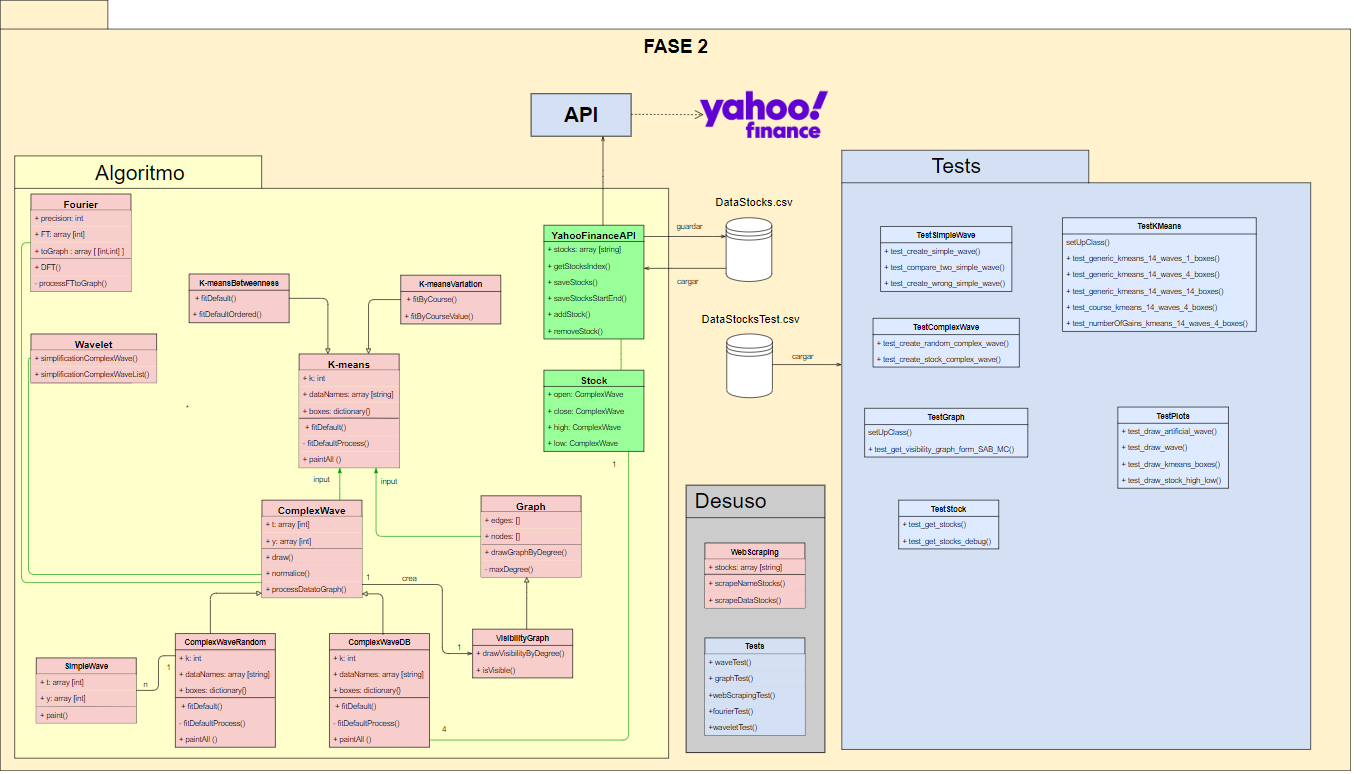
\includegraphics[width=1\linewidth]{fase 2 conexiones}
\label{fig:subrgrafo}
\end{figure}
	Creamos las estructuras que en un futuro nos servirá para realizar las simulaciones del estudio(WavePrecision y CalculateGains). Y por ultimo, la parte más importante de esta fase, modificamos la estructura del K-means utilizado buscando que nuestro algoritmo tenga resultados más consistentes que el K-means inicial. En este punto desechamos el concepto de stock que acabábamos de implementar ya que no nos es de real utilidad, y añadimos la funcionalidad de KmeansBetweenness a KmeansVariation ay que tienen la misma finalidad y con esto tenemos el back-end completo.\\
\begin{figure}[H]
\centering
  \centering
  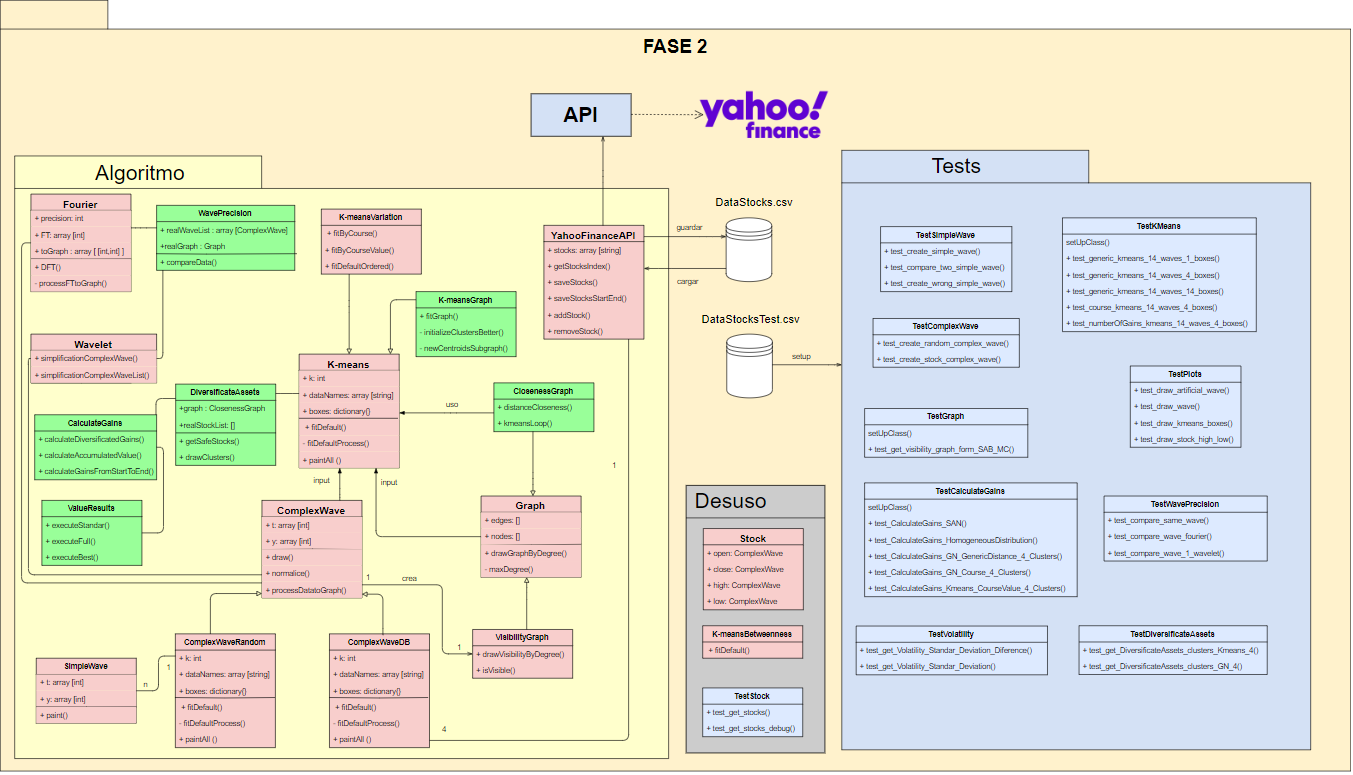
\includegraphics[width=1\linewidth]{fase 2 full}
\label{fig:subrgrafo}
\end{figure}
	\subsection{Fase 3 (Git)}
Aquí ya tenemos implementado un sistema de control de versiones Git ya que en la fase anterior dedicamos 31 horas a solucionar buggs, y eso lo podríamos haber reducido considerablemente con control de versiones:\\
\begin{figure}[H]
\centering
  \centering
  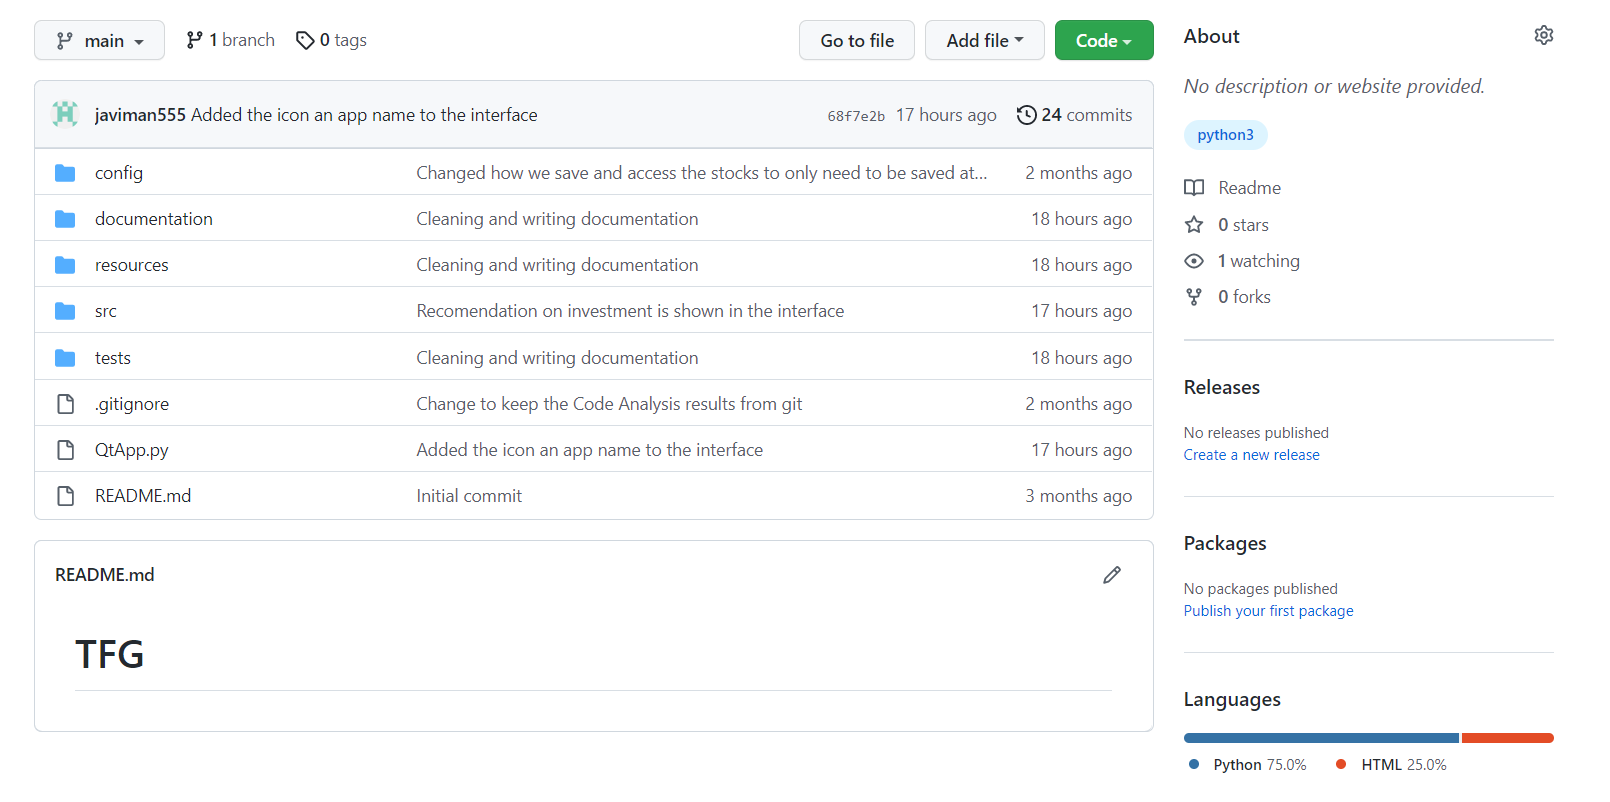
\includegraphics[width=1\linewidth]{github}
\label{fig:subrgrafo}
\end{figure}
	Engloba un periodo de 3 meses en los cuales se realizan unas 224,5 horas de trabajo distribuidas de la siguiente forma:\\
\begin{figure}[H]
\centering
  \centering
  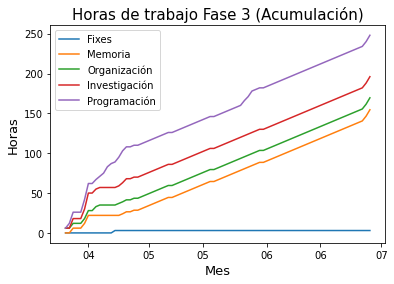
\includegraphics[width=0.5\linewidth]{tiempo fase 3}
\label{fig:subrgrafo}
\end{figure}
	En esta fase tenemos menos horas dedicadas a programación en comparación a las fases anteriores ya que el algoritmo se termino de crear en la segunda fase. En esta fase lo único que hacemos con respecto a escribir código es crear una interfaz de usuario simple y conectarla con el resto del código creando controladores para seguir una arquitectura modelo vista controlador.
\begin{figure}[H]
\centering
  \centering
  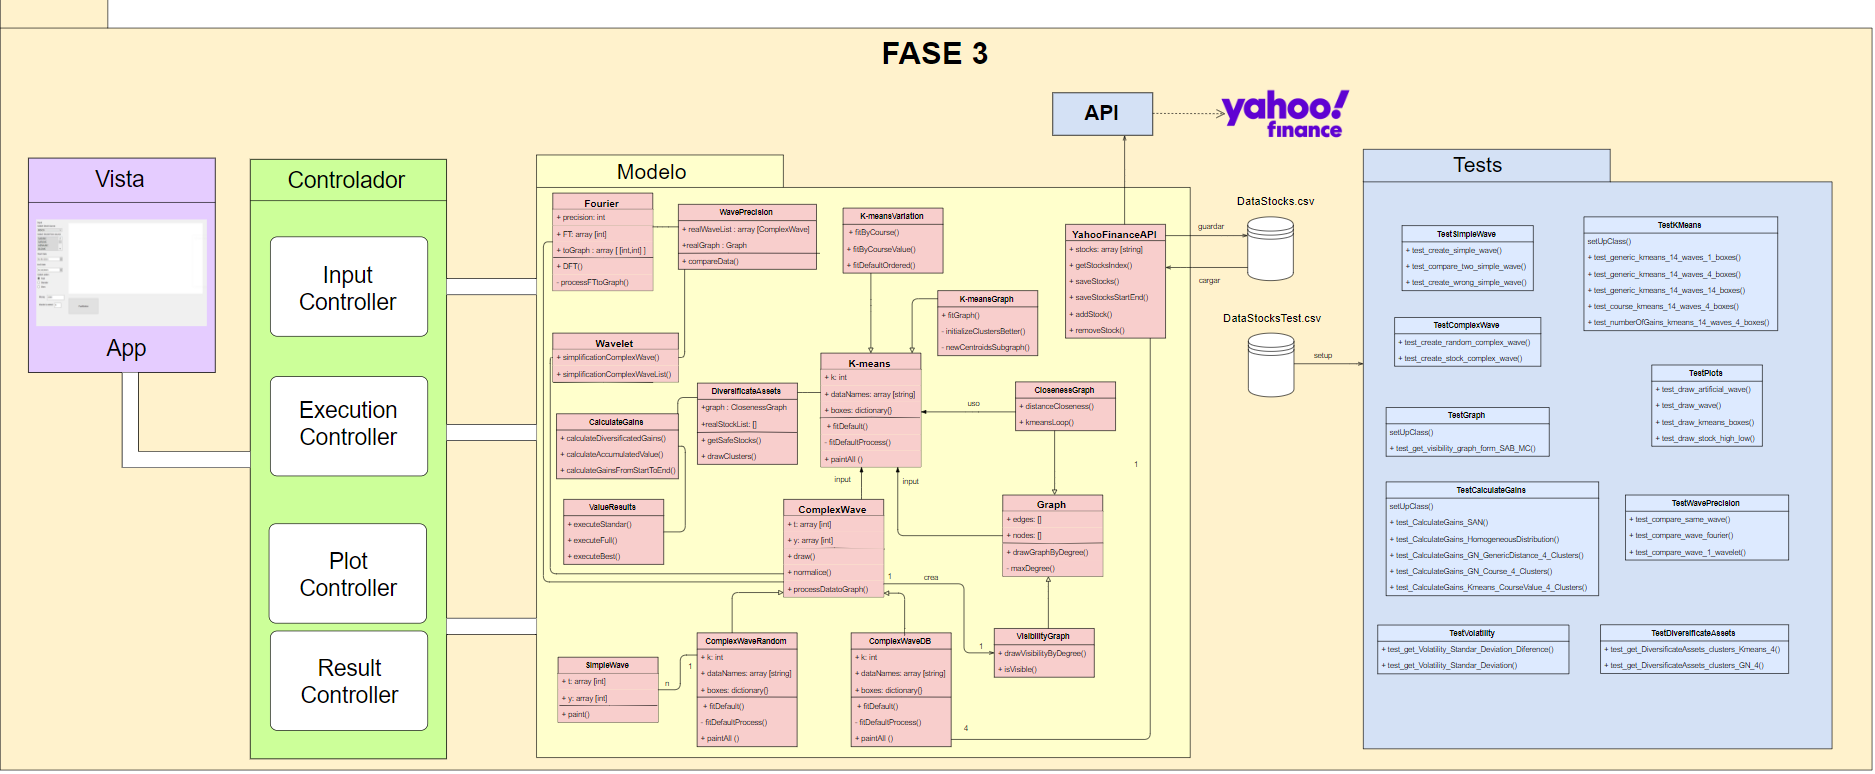
\includegraphics[width=1\linewidth]{fase 3}
\label{fig:subrgrafo}
\end{figure}
	Por otro lado a lo que más tiempo dedicamos en esta fase es a escribir las memorias del proyecto.\\
	Cabe resaltar que el tiempo dedicado a resolver buggs ha disminuido considerablemente, en parte por dedicar menos tiempo a programar,pero sin duda el control de versiones ha ayudado a mantener este numero bajo.\\
	\subsection{Casos de Uso}
	
	Ahora mostraremos el diagrama de casos de uso del programa, y a través de la interfaz mostraremos algunos ejemplos de uso.\\
\begin{figure}[H]
\centering
  \centering
  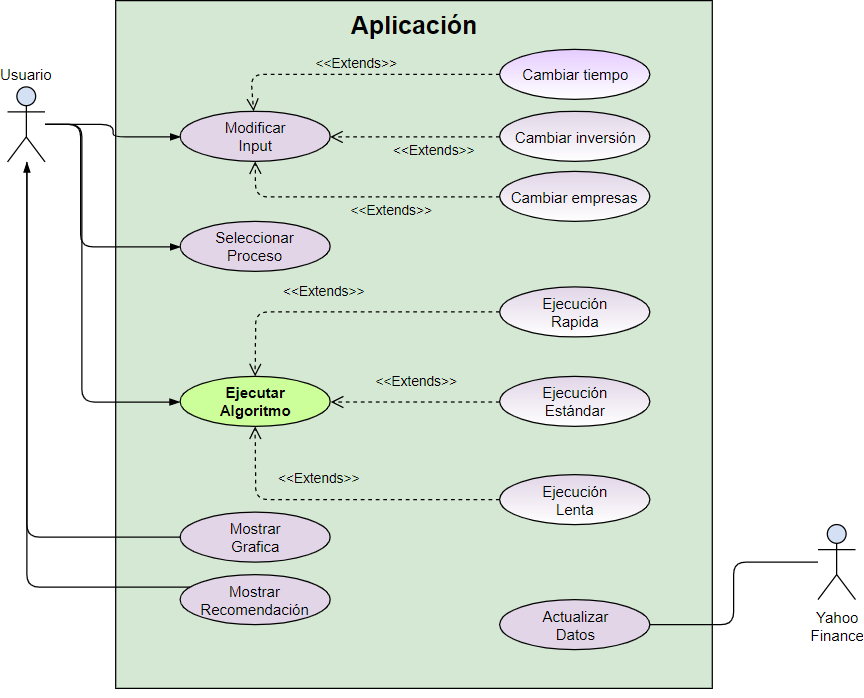
\includegraphics[width=1\linewidth]{casos de uso}
\label{fig:subrgrafo}
\end{figure}
	
	
	Primero ejecutamos la funcionalidad lenta sin modificar ninguno de los parámetros de entrada.\\
\begin{figure}[H]
\centering
  \centering
  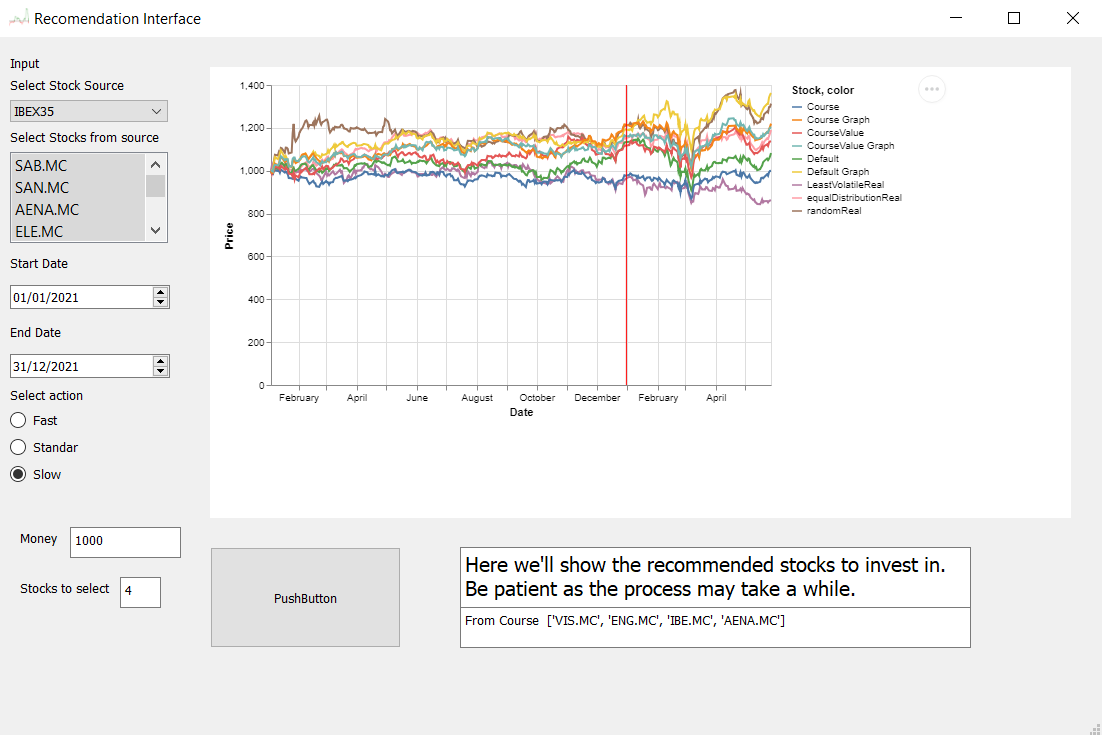
\includegraphics[width=0.5\linewidth]{execution normal}
\label{fig:subrgrafo}
\end{figure}
	Aquí vemos que nos da como recomendación 4 empresas en las que invertir y nos dice que el proceso que nos ha dado ese resultado es Course que se pude ver en cyan en la gráfica de arriba, lo que podemos hacer ahora es quitar esas empresas del input para ver que nos recomienda en su lugar.\\
\begin{figure}[H]
\centering
  \centering
  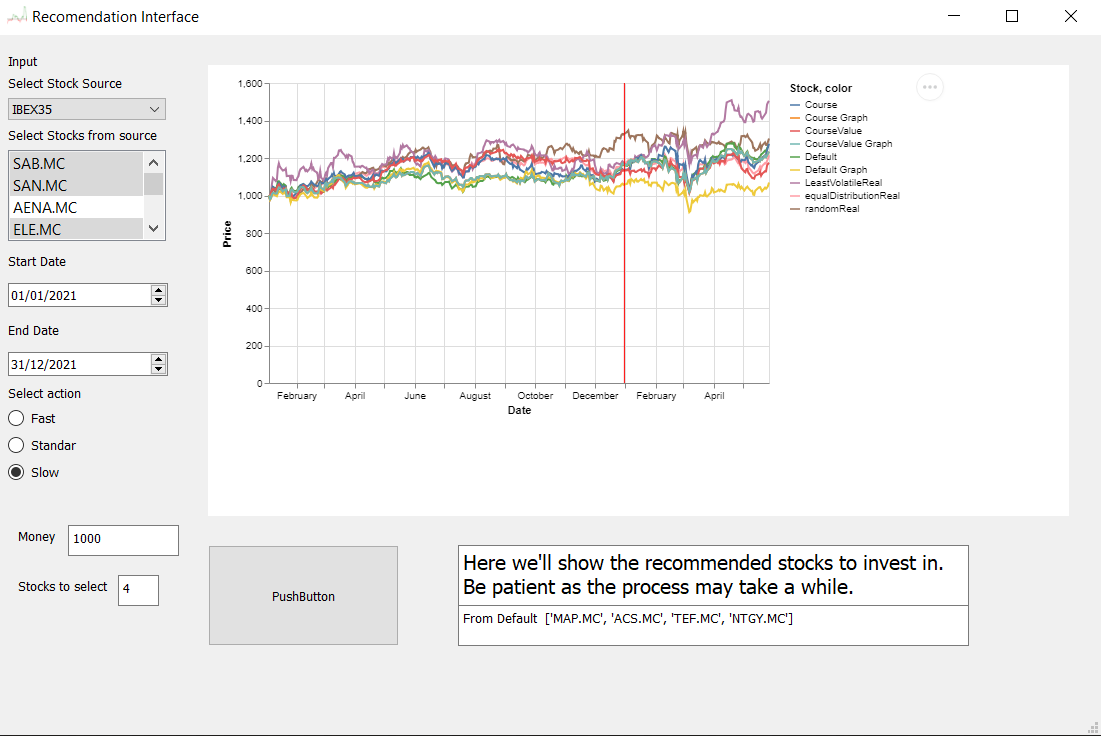
\includegraphics[width=0.5\linewidth]{execution reduce stock}
\label{fig:subrgrafo}
\end{figure}
	Podemos ver que la recomendación es distinta al no tener accesa a las empresas de la primera recomendación, por ultimo podemos probar a modificar el intervalo de tiempo y el numero de empresas a recomendar, lo que nos devuelve:\\
	\begin{figure}[H]
\centering
  \centering
  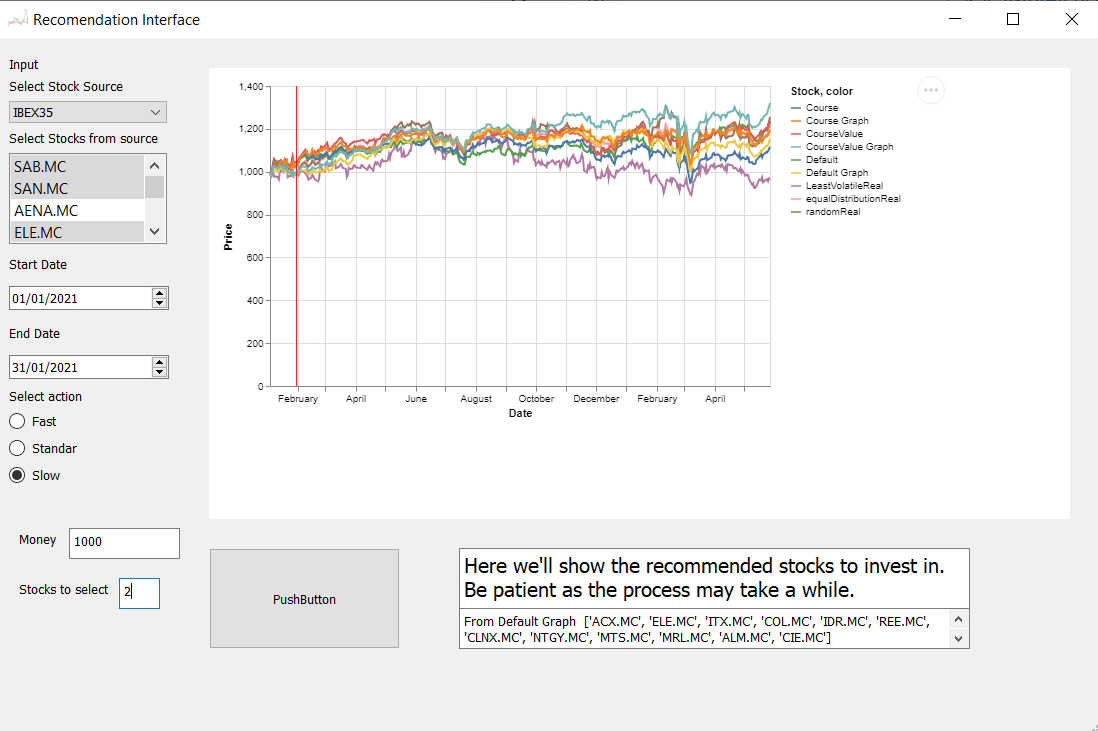
\includegraphics[width=0.5\linewidth]{execution 1 m 12 k}
\label{fig:subrgrafo}
\end{figure}
\pagebreak

	\section{Conclusiones}
	Todo este proyecto se centra en explicar los procesos y metodologías utilizadas para facilitar el código necesario para el estudio de \cite{Principal}. Posiblemente lo más relevante que se puede sacar de este desarrollo es la importancia que tiene en un proyecto software la capacidad de adaptarse a las circunstancias para mantener bajo control el desarrollo del proyecto. Sin las distintas mejoras en la metodología y arquitectura de este proyecto que se han ido implementando a lo largo del desarrollo posiblemente no se hubiera podido completar al nivel que esta ahora mismo.\\
	El proyecto ha conseguido su finalidad, proveer a \cite{Principal} el código necesario para funcionar, pero no se tiene porque parar ahí, si se sigue el desarrollo de este proyecto hay todavía mucho por mejorar en lo que respecta al desarrollo del código. A continuación se muestras algunas mejoras que se pueden implementar para mejorar el proceso software:\\
	\begin{enumerate}
	\item \textbf{Cambiar de API}: Aunque la API que hemos utilizado para recibir los datos de bolsa nos ha servido bastante bien, a lo largo del desarrollo del proyecto hemos visto inconsistencias en los datos que han limitado nuestras simulaciones. Como puede ser que a algunas empresas tienen días sin datos registrados, esto lo hemos visto en algunos datos del 2015 y para poder solventarlo deberíamos buscar alternativas pro donde coger los datos.
	\item \textbf{Tests Automáticos}: Ahora mismo los tests aunque se ejecutan todos juntos necesitan ser iniciados de forma manual, el paso siguiente en la automatización de tests es que se ejecuten cada vez que se haga un commit al repositorio y el commit solo se cumpla si pasan todos los tests.
	\item \textbf{Control de Errores}: Como su nombre indica consiste en asegurar que la aplicación funcione correctamente, y en caso contrario controlar el comportamiento inesperado de la aplicación.
	\item \textbf{Dockerizar la aplicación}: Se conoce como dockerizar al proceso de empaquetar una aplicación para su distribución y ejecución en otros ordenadores, facilitando enormemente el uso de la aplicación.
	\item \textbf{Refactorizar}: Hasta ahora hemos dejado código redundante en el proyecto para comentarlos con estas memorias, pero a partir de ahora vendría bien hacer una buena limpieza quitando los métodos que no se usen.
	\end{enumerate}
	Considero que el proyecto va por buen camino, pero tiene la capacidad de crecer mucho más.\\
	Con este trabajo dado por finalizado creo que es conveniente mostrar la grafica total del tiempo dedicado al proyecto (el script usado para crear las graficas de tiempo dedicado se puede ver en los apéndices del proyecto):
	\begin{figure}[H]
\centering
  \centering
  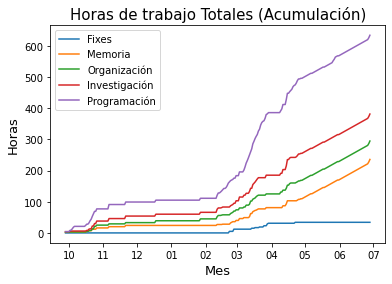
\includegraphics[width=1\linewidth]{tiempo total}
\label{fig:subrgrafo}
\end{figure}
\pagebreak
	
	\section{Bibliografía}
	 \renewcommand\refname{}
\begin{thebibliography}{X}


\bibitem{Principal} \textsc{Javier Méndez García-Brioles} \textsc{(2022)},
\textit{Proyecto principal} \url{https://github.com/javiman555/TFG/blob/main/documentation/MemoriaTFG.pdf}\\


\bibitem{MVC}Díaz González, Y., \& Fernández Romero, Y. (2012). Patrón Modelo-Vista-Controlador. Telemática, 11(1), 47–57. Retrieved from \url{https://revistatelematica.cujae.edu.cu/index.php/tele/article/view/15}
\bibitem{MVC}\textsc{José Luis Izquierdo Chávez} \textsc{(2010)},
\textit{Diseño Ágil con TDD} \url{https://d1wqtxts1xzle7.cloudfront.net/64224869/disenoAgilConTdd_ebook-with-cover-page-v2.pdf?Expires=1656449564&Signature=Fc7WEAeEIxRbM0v26pygyHRzLugbDyuB8s24OI7eLPo-U1GsBS5fgR2t4FWASO3mAPvYVoj3pflUYbNUEtN0JLMHzw2sJ5BuMntDd~qHwkTuUQ3vzbkQVGrNYkqM3V1qlgubJue-8Y7e5qDRCm77NRBZ1MKHVZR9qWBcc9suenyaaLH2U33T2E~VzW-hx4vs9nE46rDdEo~ZX3W7wTxL5adun4W68lO8d03~2eENnqxCykOn7O-6QvF1pbRQXvNe5iV0xKwMPEP~FMkUeVep59D27NZFZ871AYDvr4--HIe6fBURUNpoZ2pLDHwDWrQLjjW-Ilb4J5l2mUX0ciGcRg__&Key-Pair-Id=APKAJLOHF5GGSLRBV4ZA}\\

\bibitem{Clean Code} \textsc{Robert C. Martin}\textsc{(2008)},
\textit{Clean Code: a Handbook of Agile Software Craftsmanship
}
\bibitem{Agilidad} \textsc{Hadida, Sebastián; Troilo, Fernando}\textsc{(2020)},
\textit{La agilidad en las
organizaciones: Trabajo comparativo entre metodologías ágiles y de cascada en un contexto de
ambigüedad y transformación digital, Serie Documentos de Trabajo, No. 756, Universidad del
Centro de Estudios Macroeconómicos de Argentina (UCEMA), Buenos Aires}\url{https://www.econstor.eu/bitstream/10419/238381/1/756.pdf}

\bibitem{unitest} \textsc{Jitse Niesen}\textsc{(2014)},
\textit{Spyder-Unittest}\url{https://github.com/spyder-ide/spyder-unittest}

\end{thebibliography}
\pagebreak

\section{Apéndices}


	\textbf{Proyecto}:\url{https://github.com/javiman555/TFG}\\
	\textbf{Diagramas}: \url{https://github.com/javiman555/TFG/tree/main/resources/graphs} \\
	\textbf{Documento Exel}: \url{https://github.com/javiman555/TFG/blob/main/documentation/TFG_Horario.ods} \\
	\textbf{Trello}:\url{https://trello.com/b/erVnFgdJ/tfg}\\
	\textbf{Scripts}:\\
\pythonexternal{code/scriptTiempo.py}
\pagebreak
	\textbf{Estructura de carpetas}:\\
	\begin{figure}[H]
\centering
  \centering
  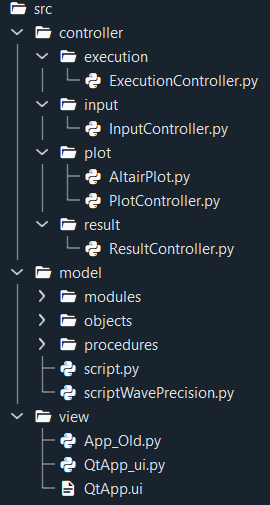
\includegraphics[width=0.5\linewidth]{carpetas modelo vista controlador}
\caption{Distribución de la estructura modelo vista controlador}
\label{fig:subrgrafo}
\end{figure}
\begin{figure}[H]
\centering
  \centering
  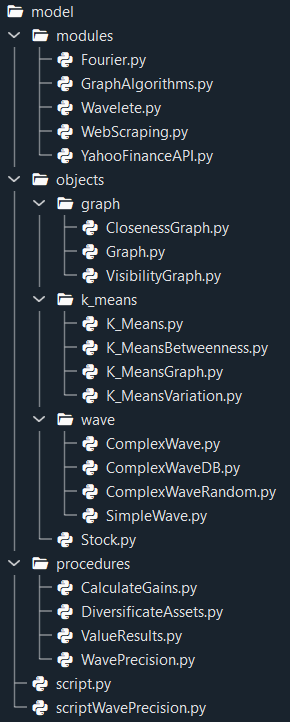
\includegraphics[width=0.5\linewidth]{carpetas modelo}
\caption{Distribución del modelo}
\label{fig:subrgrafo}
\end{figure}
\begin{figure}[H]
\centering
  \centering
  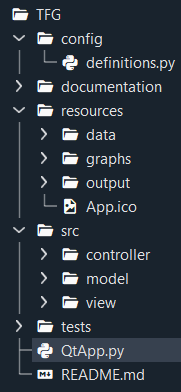
\includegraphics[width=0.5\linewidth]{carpetas proyecto}
\caption{Distribución del proyecto entero}
\label{fig:subrgrafo}
\end{figure}
\pagebreak
	

\end{document}